\chapter{Model checking for Markov decision processes} \label{model-checking-chapter}

\textit{Concepts, theorems and definitions of this chapter are essentially inspired by chapters and sections of the book ``Principles of model checking'' \cite{PMC} treating of linear temporal logic, computation tree logic, probabilistic computation tree logic and probabilistic rewards computation tree logic.}\\

In this chapter, we present a way to \textit{model-check} Markov decision processes, i.e., verify that properties hold in states of a given model.
We focus on model checking via a \textit{probabilistic branching-time logic}. We detail the syntax, the semantic and model checking algorithms of this logic.
Furthermore, we extend it to support weights of Markov decision processes, and we then formulate requests to solve
problems we encountered in the first chapter. \\ % and that we
%will address in the following chapter, covering multi-objective support for MDPs. \\

%As model checking for MDPs uses the notion of strategy to resolve nondeterminism,
%we first need to introduce this probabilistic branching time logic for MCs.

In order to introduce model checking for Markov decision processes, we first present the basic events used to form properties in this logic.
In a Markov decision process, a strategy is required to resolve nondeterminism. The events are then measured with the probability measure of the probability space defined on paths starting from a given state of the Markov chain induced by such a strategy.
We thus begin by formally introducing these events %the probabilistic branching time logic in Markov chains, before detailing these events and this logic in Markov decision processes.
and presenting a way to compute them in Markov chains, before doing the same in Markov decision processes.
%Then, we introduce a probabilistic branching time for Markov chains and Markov decision processes, and

\section{Temporal events}\label{tempevent}
In Markov chains, \textit{temporal events} allow to describe %\textit{quantitative} and \textit{qualitative}
properties related to the reachability to a set of target states in the system. These properties are classified into two categories: \textit{quantitative} and \textit{qualitative} properties.
Quantitative properties may assert the probability to reach a subset of target states, avoiding some bad states in an infinite or finite number of steps, and
qualitative properties are special cases of quantitative properties where probabilities are trivial (i.e., zero or one).
%In order to describe these temporal events, we use \textit{LTL-like} notations.
%\textit{Linear temporal logic} (LTL) is a logical formalism
%that is suited for specifying linear temporal properties.
%In PCTL, notations of linear temporal operators (cf. Figure \ref{ltl}) are actually derived from LTL temporal operators, dealing with paths of any system.
%For example, following a subset of target states $T \subseteq S$ of the system, the event of reaching $T$ is denoted by $\Diamond T$ that is defined with a finite union of cylinder sets, ensuring its measurability.
%We will define here some temporal events, that are actually used to form PCTL path formulae events. So, we need to ensure their measurability.
We present in this section a way to determine the probability of events describing such properties, which will be useful later to model-check Markov chains and Markov decision processes in a probabilistic branching time logic.
\subsection{Constrained reachability}
\begin{definition}[\textbf{Constrained reachability events}]
Let $\mathcal{M}$ be an MC with state space $S$, $s \in S, \, T, C \subseteq S$, and $n \in \mathbb{N}$. The events $C \U^{\leq n} \, T$ and $C \U T$ are sets of paths starting from $s$ describing the constrained reachability by the set of states $C$ to the set of target states $T$.
These events are defined as follows:
\begin{align*}
  C \U^{\leq n} \, T &= \{ s_0 s_1 s_2 \dots \in Paths(s) \; | \; \exists j \leq n, \, s_j \in T, \, \text{and } \forall i < j,\, s_j \in C \}, \\
  C \U T &= \{ s_0s_1s_2 \dots \in Paths(s) \; | \; \exists j \in \mathbb{N}, \, s_j \in T, \, \text{and } \forall i < j, \, s_j \in C \}.
\end{align*}
Their notation is inspired by \textit{PCTL} (a probabilistic branching time logic, cf. Section \ref{pctl-section}).
\end{definition}

\begin{lemma}[Measurability of the constrained reachability events] \label{cut-lemma}
  Let $\mathcal{M}$ be an MC with state space $S$, $s \in S$, $C, T \subseteq S$, and $n \in \mathbb{N}$.
  The events $C \U^{\leq n} \, T$ and $C\U T$ are measurable.
\end{lemma}

\begin{proof2}
  The events $C \U^{\leq n} \, T$ and $C\U T$ are measurable since they can be defined as countable union of cylinder sets:
  \begin{align*}
    C \U^{\leq n} \, T &= \bigcup_{k=0}^n\,\bigcup_{s_0\dots s_k \in Paths_{fin}^{C,\, k,\, T}(s)} Cyl(s_0\dots s_k),\\
    C \U T &= \bigcup_{k\in \mathbb{N}}\,\bigcup_{s_0\dots s_k \in Paths_{fin}^{C,\, k,\, T}(s)} Cyl(s_0\dots s_k)
  \end{align*}
  where $n \in \mathbb{N}$, and \[Paths_{fin}^{C,\, n,\, T}(s) = \{ s_0 \dots s_n \in Paths_{fin}(s) \; | \; \forall i < n, \, s_i \in C \setminus T \; \wedge s_n \in T\}.\]
  $\mathbb{P}_s(C \U^{\leq n} \, T)$ and $\mathbb{P}_s(C \U T)$ denote the probability of the union of cylinder sets of finite paths  of $Paths_{fin}^{C, \, k, \, T}(s)$ starting from the state $s \in S$.
\end{proof2}
$ $ \\

The constrained reachability event allows to derivate some other classical events:
\begin{itemize}
  \item $\Diamond T = S \U T$, i.e., \textit{reach $T$} (cf. Subsection \ref{obj-MC} in the first chapter),
  \item $\Diamond^{\leq n}\, T = S \U^{\leq n}\, T$, i.e., reach $T$ \textit{in at most $n$ steps},
  \item $\Box T =  \overline{\Diamond \overline{T}}$,
  %$ \; \implies \; \mathbb{P}_s(\Box T) = 1 - \mathbb{P}_s (\Diamond (S \setminus T))$
  i.e., \textit{always visit $T$},
  \item $\Box^{\leq n} T =  \overline{\Diamond^{\leq n} \overline{T}}$,
  %$ \; \implies \; \mathbb{P}_s(\Box T) = 1 - \mathbb{P}_s (\Diamond (S \setminus T))$
  i.e., \textit{repeat $T$ at least $n$ times}.
\end{itemize}

In order to compute the probability of such events, it is sufficient to compute the probability of the constrained reachability.\\

Let $s \in S$, $C, T \subseteq S$, and $n \in \mathbb{N}$. In order to compute $\mathbb{P}_s(C \U^{\leq n} \, T)$ and $\mathbb{P}_s(C \U T)$, we introduce the following notations.
Let $S_{=0}$, $S_{=1}$ and $S_{=?}$ be partitions of $S$ such that
\begin{itemize}
  \item $T \subseteq S_{=1} \subseteq \{s \in S \; | \; \mathbb{P}_s(C \U T) = 1\}$,
  \item $S \setminus (C \cup T) \subseteq S_{=0} \subseteq \{ s \in S \; | \; \mathbb{P}_s(C \U T) = 0 \}$,
  \item $S_? = S \setminus (S_{=1} \cup S_{=0})$.
\end{itemize}
Then, let $A$ be a quadratic matrix with rows and columns referring the states of $S_?$. This matrix is obtained from the transition function $\Delta$ as follows:
\[
  A_{i, j} = \Delta(s_i, s_j) \quad \forall s_i, s_j \in S_?
\]
Let $n_?$ = $|S_?|$. Similarly, let $b$ be a vector of probabilities in $[0, 1]^{n_?}$ , defined as $(b_s)_{s \in S_?}$ such that $b_s = \sum_{t \in S_{=1}} \Delta(s, t)$, i.e., such that $b_s$ describes the probability of reaching a state of $S_{=1}$ in one outgoing transition of the state $s$.

\begin{notation}[\textit{Lifted probability transition}]
  Let $s \in S$ be a state of $\mathcal{M}$. We denote by $\Delta(s, T)$ the probability of reaching $T$ in one outgoing transition of $s$, i.e., $\Delta(s, T) = \sum_{t \in T} \Delta(s, t)$.
\end{notation}
\noindent So, we have $b_s = \Delta(s, S_{=1})$ for each $s \in S_?$.
\begin{theorem}[\bfseries\itshape Least fixed point characterisation for constrained reachability]\label{theoCUT}
  Let $x$ be a vector of probabilities in $[0,1]^{n_?}$ such that $x=(\mathbb{P}_s(C \U T))_{s \in S_?}$. This vector is the
  \textit{least fixed point} of the operator $\Upsilon : [0, 1]^{n_?} \rightarrow [0, 1]^{n_?}$ which is given by %Let $(y_s)_{s \in S_?} \in [0, 1]^{n_?}$, the least fixed point of the operator $\Upsilon$ is given by
  \[
    \Upsilon(y) = A y + b
  \]
  Furthermore, let $x^{(0)} = \vec{0}$ be the vector consisting of zeros only and $x^{(n+1)} = \Upsilon(x^{n})$ for $n \in \mathbb{N}$, then
  \begin{itemize}
    \item $x^{(n)} = (x_s^{(n)})_{s \in S_?}$, where $x_s^{(n)} = \mathbb{P}_s(C \U^{\leq n} S_{=1})$ for each state $s \in S_?$,
    \item $x^{(0)} \leq x^{(1)} \leq x^{(2)} \leq \dots \leq x$, and
    \item $x = \lim_{n\rightarrow\infty}x^{(n)}$.
  \end{itemize}
  where $\leq$ denotes here the partial order relation \[\leq \,=\, \{ (y, y') \in [0, 1]^{n_?} \times [0,1]^{n_?} \; | \; y_s \leq y'_{s} \;\; \forall s \in S_?\}.\]
\end{theorem}
\noindent By definition of $A$ and $b$, for any $s \in S_?$ and for $y = (y_s)_{s \in S_?} \in [0, 1]^{n_?}$,
\[
  (\Upsilon(y))_s = y'_s = \sum_{s' \in S_?} \Delta(s, s') \cdot y_{s'} + \Delta(s, S_{=1}).
\]
Since $0 \leq y_s \leq 1$ for all $s \in S?$,
$\Delta(s,s') \geq 0$, and $\sum_{s' \in Succ(s)}
\Delta(s, s')=1$, this implies $0 \leq y_{s'}\leq 1$.
We then have that $\Upsilon$ is a well-defined function from $[0, 1]^{n_?}$ to $[0, 1]^{n_?}$.
Furthermore, let $x_s = \mathbb{P}_s(C \U T)_{s \in S_?}$ for each state $s \in S$, by definition of $\Upsilon$, we intuitively have
\begin{flalign}
  x^{(0)} &= \vec{0}, \notag \\
  x^{(1)} &= A x^{(0)} + b \notag \\
          &= b, \tag{\itshape states of $C$ reaching $S_{=1}$ in one transition}\\
  x^{(2)} &= A x^{(1)} + b \notag \\
          &= A b + b \notag \\
          &= (\sum_{s' \in S_?} \Delta(s, s') \cdot \Delta(s', S_{=1}) + \Delta(s, S_{=1}))_{s \in S_?} \tag{\itshape states of $C$ reaching $S_{=1}$ in max. two transition steps} \\
  \dots& \notag \\
  x^{(n)} &= A x^{(n-1)} + b \tag{\itshape states of $C$ reaching $S_{=1}$ in max. $n$ transition steps} \\
  &= A^{n-1} b + A^{n-2} b + \dots + Ab + b \notag \\
  \dots &\notag \\
  x &= Ax+b \notag \\
  x &= (\sum_{s' \in S} \Delta(s, s') \cdot x_{s'} + \Delta(s, S_{=1}))_{s \in S_?} \tag{\itshape states of $C$ eventually reaching $S_{=1}$}
\end{flalign}
\begin{remark}[\textit{Choosing $S_{=0}$ and $S_{=1}$}]\label{remarkS0S1}
For efficiency reasons, it is a good idea to deal with the largest subsets $S_{=0}$ and $S_{=1}$. Indeed, this allows to reduce
the size of the matrix $A$ and allows faster computations to determine the probability of constrained reachability events.
However, under the assumption that $S_{=0}$ is a proper subset of $\{ s \in S \; | \; \mathbb{P}_s(C \U T) = 0 \}$, the operator $\Upsilon$ may have more than one fixed point.
%, and
%we thus need to deal with the largest set $S_{=0}$ as possible, i.e., $S_{=0} = \{ s \in S \; | \; \mathbb{P}_s(C \U T) = 0 \}$.
Let $\mathcal{M}$ be the MC of Figure \ref{s0s1} and $T = \{t\}$.
\begin{figure}[h]
  \centering
  
\includegraphics[width=0.3\linewidth]{resources/S0S1}
  \caption{Markov chain $\mathcal{M}$ with $2$ states : $s$ and $t$}\label{s0s1}
\end{figure}
Consider the event $\Diamond T$. Let us take the smallest subsets $S_{=1} = T$ and $S_{=0} = S \setminus (S \cup T) = \emptyset$, thus $S_? = S \setminus T = \{s\}$. Following Theorem \ref{theoCUT}, let $x = (\mathbb{P}_s(C \U T))_{s \in S_?}$, where $x = Ax+b$. As $x=x_s$ and $b = 0$ (because $\Delta(s, t) = 0$),
we have $x = Ax$, with $A = 1$ (because $\Delta(s, s) = 1$). The related operator $\Upsilon:[0, 1] \rightarrow [0,1]$ is given by $\Upsilon(y_s) = y_s$ for any $y_s \in [0, 1]$ and has then infinitely many fixed points.
\end{remark}
% \begin{definition}[\textbf{Paths satisfiability of $C \U T$ events}]
%   Let $\mathcal{M}=(S, \Delta, w, AP, L)$ be an MC, $T, C \subseteq S$ and $\pi \in Paths(s)$ be a path starting from any $s \in S$. The path $\pi$ satisfies the event $C \U T$ iff
% \end{definition}
The unicity of the fixed point is actually guaranteed if $\mathcal{M}$ is finite and if we take the largest subset for $S_{=0}$, i.e., $S_{=0}=\{s \in S \; | \; \mathbb{P}_s(C \U T) =0 \}$.

\begin{theorem}[\bfseries\itshape Unique solution for the constrained reachability] \label{unique-sol}
Let $\mathcal{M}$ be a Markov chain with state space $S$, the subsets $T, C \subseteq S$,
\[
  S_{=0} = \{s \in S \; | \; \mathbb{P}_s(C \U T) = 0 \}, \quad
  T \subseteq S_{=1} \subseteq \{s \in S \; | \; \mathbb{P}_s(C \U T) = 1 \},
\]
and $S_? = S \setminus (S_{=0} \cup S_{=1})$. Then , the vector $(\mathbb{P}_s(C \U T))_{s \in S_?}$ is the unique fixed point of $\Upsilon$ and the unique solution of the equation system $x = Ax+b$, where $A = (\Delta(s, s'))_{s, s' \in S_?}$ and $b = (\Delta(s, S_{=1}))_{s \in S_?}$.
\end{theorem}

\begin{remark}[\textit{Reachability problem}]
  Remind the reachability problem addressed in the first chapter (i.e., computing $\mathbb{P}_s(\Diamond T)$ for a subset of target states $T$ and for any $s \in S$, cf. Subsection \ref{obj-MC}), the linear equations system resolving the problem (cf. Appendix \ref{app-reach}) is actually derived from Theorem \ref{unique-sol}.
\end{remark}

\begin{remark}[\textit{Probability of the always event}]
  Let $\mathcal{M}$ be an MDP with state space $S$ $s \in S$, and $T \subseteq S$, the event $\Box T$ is equal to $\overline{\Diamond \overline{T}}$.
  Since we can compute $\mathbb{P}_s(S \U \overline{T}) = \mathbb{P}_s(\Diamond \overline{T})$ (cf. Theorem \ref{unique-sol}), we have $\mathbb{P}_s(\Box T) = 1 - \mathbb{P}_s(\Diamond (S \setminus T))$.
\end{remark}

We now provide a way to compute the largest subset $S_{=0}$. Note that we will also see later a way to compute the largest subset $S_{=1}$ in order to allow faster computations to solve the system of  equations defined in Theorem \ref{unique-sol} (cf. Corollary \ref{qualitative-const-reach}).

\begin{definition}[\textbf{Paths satisfiability relation with constrained reachability events}]
Let $\mathcal{M}$ be an MC with state space $S$ and $\pi \in Paths(s)$ be a path starting from any state $s \in S$. The path $\pi$ \textit{satisfies} $C \U T$ iff there exists a prefix $\hat{\pi}\in Pref(\pi)$ and a number of steps $k \in \mathbb{N}$ such that $\hat{\pi} \in Paths_{fin}^{C,\, k,\, T}(s)$. This relation is denoted by $\models$, with $\pi \models C \U T$.
\end{definition}
\begin{lemma}[Zero probability equivalence of constrained reachability events] Let $s \in S$ be a state in an MC with state space $S$ and $C, T \subseteq S$, the two following propositions are equivalent:
  \begin{enumerate}[(a.)]
    \item $\mathbb{P}_s(C \U T) = 0$. \label{p1}
    \item $\forall \pi \in Paths(s), \, \pi \not \models (C \U T)$. \label{p2}
  \end{enumerate}
\end{lemma}

 \begin{proof2}$ $\\
    ($\ref{p2}\implies\ref{p1}$). Assume that $\forall \pi \in
    Paths(s)$, $\pi \centernot\models C \U T$. So, by definition of the satisfaction relation $\models$, that
    means there does not exist any finite path $\hat{\pi} \in
    Paths_{fin}(s)$ such that
    $\hat{\pi} \in Paths_{fin}^{C, \, k,\, T}(s)$ for some $k \in \mathbb{N}$. By definition
    of $C \U T$, that implies $C \U T = \emptyset$ and then
    $\mathbb{P}_s(\emptyset) = 0$.\\
    ($\neg\ref{p2}\implies\neg\ref{p1}$). Assume there exists a path $\pi \in Paths(s)$ such that $\pi \models C \U T$.
    Then, that means there exists a prefix $\hat{\pi} = s_0 \dots s_k \in Pref(\pi)$ and a number of steps $k \in \mathbb{N}$ such that
    $\hat{\pi} \in Paths_{fin}^{C, \, k, \, T}(s)$. So, we have at least one cylinder set in the union forming the event $C \U T$ (i.e., $Cyl(s_0\dots s_k)$), and then $\mathbb{P}_s(C \U T) \geq \prod_{i = 0}^{k-1} \Delta(s_i , s_{i+1}) > 0$.
 \end{proof2}

\begin{lemma}[Computing $S_{=0}$ with graph theory]\label{S0graph}
Let $s \in S$ be a state in an MC with state space $S$ and $C, T \subseteq S$,
  the statement $\forall \pi \in Paths(s), \, \pi \centernot \models (C \U T)$ can be decided in polynomial time in the size of $\mathcal{M}$ with a graph theory based algorithm.
\end{lemma}

\begin{proof2}
The set $B = \{ s \in S \; | \; \exists \pi \in Paths(s), \;\; \pi \models (C \U T) \}$ is the smallest subset of $S$ such that
\begin{enumerate}[(a.)]
  \item $T \subseteq B$, and \label{gtproof1}
  \item $\forall s \in S, \; s \in C \; \wedge \; Succ(s) \cap B \neq \emptyset \implies s \in B$. \label{gtproof2}
\end{enumerate}
Indeed,
\begin{enumerate}
  \item Assume that $B = \{s \in S \; | \; \exists \pi \in Paths(s), \; \pi \models C\U T\}$ and let us show that $B$ satisfies \ref{gtproof1} and \ref{gtproof2}. We obviously have that $T \subseteq B$ because all paths starting from $t \in T$ satisfies $C \U T$: take the finite path consisting in the single state $t$, we have that
  $t \in Paths_{fin}^{C, \, 0,\, T}(t)$.
  Then, let $s \in S$ and assume that $s \in C \setminus T$ and $Succ(s) \cap B \neq \emptyset$. That means there exists a successor $s'$ of $s$ such that $s' \in B$. Thus, there exists
  a path $\pi \in Paths(s')$ such that $\pi \models C\U T$, by definition of $B$. Furthermore, we have by definition of the satisfaction relation $\models$ that there exists a prefix $\hat{\pi}\in Pref(\pi)$ and a steps number $k \in \mathbb{N}$ such that $\hat{\pi} \in Paths_{fin}^{C, \, k,\, T}(s')$. So, let take the finite path $s.\hat{\pi}$, we have that $s.\hat{\pi} \in Paths^{C, \, k+1, \, T}_{fin}(s)$
  and thus that $s.\pi \models C \U T$. That yields $s \in B$.
  \item Let $B \subseteq S$ be the smallet set satisfying \ref{gtproof1} and \ref{gtproof2}.
  Let us show that $\{s \in S \; | \; \exists \pi \in Paths(s), \; \pi \models C\U T\} \subseteq B$.
  %Assume that $T \subseteq B$ and that if we have $s \in C \; \wedge \; Succ(s) \cap B \neq \emptyset$, then we have $s \in B$.
  First, if $\{s \in S \; | \; \exists \pi \in Paths(s), \; \pi \models C \U T\} = \emptyset$,
  then we trivially have that our assumptions are verified. Then, assume that $\{s\in S \; | \; \exists \pi \in Paths(s), \; \pi \models C \U T\} \neq \emptyset$ and let $s \in \{s\in S \; | \; \exists \pi \in Paths(s), \; \pi \models C \U T\}$. If $s \in T$, then $s \in B$ by \ref{gtproof1}.
  Else, we have that there exists a path $\pi = s_0 s_1 s_2 \dots \in Paths(s)$ starting from the state $s_0=s$ such that  $\pi \models C \U T$.
  By definition of the satisfaction relation $\models$, that means there exists
  $\hat{\pi} \in Pref(\pi)$ and a number of steps $k \in \mathbb{N}$ such that $\hat{\pi} \in Paths_{fin}^{C, \, k, \, T}(s)$, i.e., such that $\forall i \in \mathbb{N}$, $i < k$, $s_i \in C \setminus T$ and $s_k \in T$.
% \begin{itemize}
%   \item If $s_1 \in T$, then $s_1 \in B$, and $s_0=s \in B$ by our assumptions.
    %\item
    Let $i \in \{0, \dots, k-1\}$.
    Assume that $s_{i+1} \in B$. Then, since $s_i \in C$ and $s_{i+1} \in Succ(s_i)$, we have $s_i \in B$ by \ref{gtproof2}.
%  \end{itemize}
  Since $s_k \in T$ and $T \subseteq B$, we have by induction (from $k$ to $0$) on $i$ that $s_0=s \in B$.
  Thus, we finally have that $\{s \in S \; | \; \exists \pi \in Paths(s), \; \pi \models C \U T\} \subseteq B$.
\end{enumerate}
Then, we can compute the set $B$ with the following algorithm:
\begin{algorithm}[H]
\caption{Smallest fixed point computation}
\begin{algorithmic}[1]
  \REQUIRE a Markov chain $\mathcal{M}$ with state space $S$, and $C, T \subseteq S$
  \ENSURE the set $\{ s \in S \; | \; \exists \pi \in Paths(s), \;\; \pi \models (C \U T) \}$
  \STATE $B \leftarrow T$
  \WHILE{$A \leftarrow \{ s \in C \setminus B \; | \; Succ(s) \cap B \neq \emptyset \} \neq \emptyset$}
    \STATE $B \leftarrow B \cup A$
  \ENDWHILE
  \RETURN $B$
\end{algorithmic}
\end{algorithm}
Finally, the set \[\{s \in S \; | \; \mathbb{P}_s(C \U T) = 0 \} = \{s \in S \; | \; \forall \pi \in Paths(s), \; \pi \centernot \models (C \U T) \}\] is equal to $S \setminus B$.
\end{proof2}

\begin{example}[\textit{Constrained reachability of an MC modelling the production of solar panels according to weather}]
Let $\mathcal{M}_{sp} = (S, \Delta, w, AP, L)$ be the MC of Figure \ref{solarpanel} (cf. Example \ref{solar-panel} in the first chapter for more details about this MC).
  \begin{figure}[h!]
    \centering
    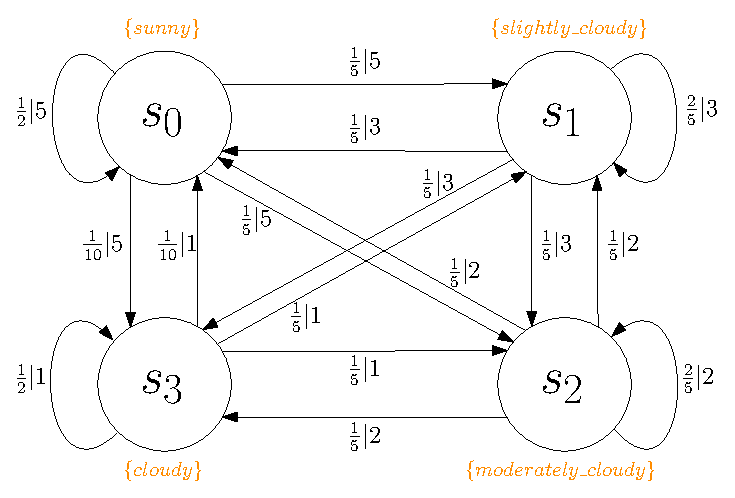
\includegraphics[width=0.5\linewidth]{resources/weather-solar-pannel}
    \captionsetup{justification=centering}
    \caption{MC modelling a daily production of energy (in $kJ$) of solar panels according to weather}
    \label{solarpanel}
  \end{figure}
  We are interested to know the probability that the weather goes from sunny to cloudy in at most three days
  (starting on a sunny day), i.e., $\mathbb{P}_{s_0}(\{s_0\} \U^{\leq 2} \{s_3\})$.
  Let $S_{=1} = \{s_3\}$ and $S_{=0} = \{ s_1, s_2 \}$, we have $S_? = \{s_0\}$. The least fixed point characterisation suggests the following iterative scheme:
  \begin{itemize}
    \item $x^{(0)} = 0$,
    \item $x^{(1)} = \Delta(s_0, s_0) \cdot x^{(0)} + \Delta(s_0, s_3) = \frac{1}{10},$ and
    \item $x^{(2)} = \Delta(s_0, s_0) \cdot x^{(1)} + \Delta(s_0, s_3) = \frac{1}{2} \cdot \frac{1}{10} + \frac{1}{10} = \frac{3}{20}$,
  \end{itemize}
  with $x^{(2)} = \mathbb{P}_{s_0}(\{s_0\} \U^{\leq 2} \{s_3\})$.
\end{example}
\begin{example}[\textit{Measuring constrained reachability event in an MC}] \label{constrained-reach-example}
Let $\mathcal{M}=(S, \Delta)$ be the MC of Figure \ref{CUTexample},
 $C = \{s_0, s_2, s_3\}$ and $T = \{s_1\}$. We are interested in the probability of the constrained reachability $C \U T$.
  \begin{figure}[H]
    \centering
    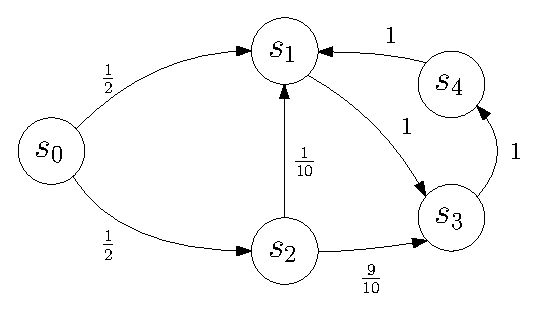
\includegraphics[width=0.4\linewidth]{resources/CUTexample}
    \captionsetup{justification=centering}
    \caption{MC $\mathcal{M}$ with state space $S = \{s_0, s_1, s_2, s_3, s_4\}$}\label{CUTexample}
  \end{figure}
  Let $S_{=1} = \{s_1\}$ and $S_{=0} = \{s \in S \; | \; \mathbb{P}_{s}(C\U T)=0\} = \{s_3, s_4\}$, we have $S_{?} = \{s_0, s_2\}$.
  The vector $(\mathbb{P}_{s}(C \U T))_{s \in S_?}$ is the unique solution of the following system:
  \begin{align*}
  	\begin{pmatrix}
      x_{s_0}\\[0.3em]
      x_{s_2}
  	\end{pmatrix} &=
    \begin{pmatrix}
      0 & \frac{1}{2} \\[0.3em]
      0 & 0
    \end{pmatrix}
    \begin{pmatrix}
      x_{s_0}\\[0.3em]
      x_{s_2}
    \end{pmatrix}
    +
    \begin{pmatrix}
      \frac{1}{2}\\[0.3em]
      \frac{1}{10}
    \end{pmatrix} \\
    \begin{pmatrix}
      x_{s_0}\\[0.3em]
      x_{s_2}
  	\end{pmatrix} &=
    \begin{pmatrix}
      \frac{1}{2} x_{s_2} \\[0.3em]
      0
    \end{pmatrix}
    +
    \begin{pmatrix}
      \frac{1}{2}\\[0.3em]
      \frac{1}{10}
    \end{pmatrix}
  \end{align*}
  So, $\mathbb{P}_{s_2}(C \U T) = x_{s_2} = \frac{1}{10}$ and $\mathbb{P}_{s_0}(C \U T) = x_{s_0} = \frac{11}{20}$.
  \\
\end{example}

In order to optimise the resolution of systems of linear equations defined to compute the probabilities of constrained reachability events,
we need to compute the largest subset $S_{=1}$, and this can be done by looking at the limit behaviour of Markov chains.

\subsection{Limit behaviour of Markov chains}\label{temp-event-mdp}
Now, we will focus on events characterising the \textit{long-run} behaviour of Markov chains. We will address here two events : $\Box\Diamond T$ ($T$ is reached \textit{infinitely often})
and $\Diamond \Box T$ ($T$ is \textit{persistent}), for any subset of states $T \subseteq S$.
We begin by defining these events and show that they are measurable. After that, we introduce some graph theory notions, allowing to study the limit behaviour of Markov chains.
Studying the limit behaviour of Markov chains allows to optimise
computations during the resolution of problems requiring linear equations systems or linear programs. Moreover, it allows fast computations to determine probabilities of \textit{infinitely often} and \textit{persistent} events.

\begin{definition}[\textbf{Infinitely often event}]
  Let $\mathcal{M}$ be an MC with state space $S$, $s \in S$, and $T \subseteq S$ be a subset of states of $\mathcal{M}$. For any path $\pi = s_0 s_1 s_2 \dots \in Paths(s)$,
encountering \textit{infinitely often} $T$ actually means that, for all step $n \in \mathbb{N}$ (and thus, for any state $s_n$ of $\pi$), there exists a state such that $s_m \in T$, with $m \geq n$.
Then, the infinitely often event for $T$ is defined as follows:
\[
  \Box\Diamond T = \{ s_0 s_1 s_2 \dots \in Paths(s) \; | \; \forall n \in \mathbb{N}, \, \exists m \geq n, \, s_m \in T \}.
\]
\end{definition}

\begin{definition}[\textbf{Persistence event}]
  Let $\mathcal{M}$ be an MC with state space $S$, $s \in S$, and $T \subseteq S$ be a subset of states of $\mathcal{M}$.
  For any path $\pi = s_0 s_1 s_2 \dots \in Paths(s)$,
 $T$ is \textit{persistent} actually means there exists a step $n \in \mathbb{N}$ such that, for all $i\geq n$, $s_i \in T$. The persistence event for $T$ is defined as follows:
 \[
  \Diamond \Box T = \overline{\Box \Diamond (S \setminus T)}.
 \]
\end{definition}

\begin{lemma}[Measurability of infinitely often events and persistence events]
Let $\mathcal{M}$ be an MC with state space $S$, $s \in S$, and $T \subseteq S$ be a subset of states of $\mathcal{M}$. The events $\Box\Diamond T$ and $\Diamond \Box T$ are measurable.
\end{lemma}

\begin{proof2}
Let
  \begin{align*}
    Paths_{fin}^{m,\, T}(s) &= \{ s_0\dots s_m \in Paths_{fin}(s) \; | \; s_m \in T \}, \text{ and} \\
    Cyl^{m,\, T}(s) &= \bigcup_{s_0 \dots s_m \in Paths_{fin}^{m, \, T}(s)} Cyl(s_0\dots s_m)
  \end{align*}
  for any $m \in \mathbb{N}$.
  The infinitely often event for $T$ can be defined as a countable intersections and unions of cylinder sets:
  \[
    \Box \Diamond T = \bigcap_{n \in \mathbb{N}} \bigcup_{m \geq n} Cyl^{m, \, T}(s).
  \]
  This event is thus measurable, and $\mathbb{P}_s(\Box\Diamond T)$ denotes the probability measure of this event. Since $\Box \Diamond (S \setminus T)$ is measurable, $\Diamond \Box T$ is measurable, with \[\mathbb{P}_s(\Diamond \Box T) = 1 - \mathbb{P}_s(\Box \Diamond (S \setminus T)).\]
\end{proof2}
$ $\\

We now provide a way to compute the probability of these events with graph theory algorithms. To do that, we need to introduce some graph concepts.

\begin{definition}[\textbf{Bottom strongly connected components}]
Let \sloppy$\mathcal{M}=(S, \Delta, w, AP, L)$ be an MC and $T \subseteq S$ be a subset of states of $\mathcal{M}$.
\begin{itemize}
  \item $T$ is \textit{strongly connected} if for any $s, s' \in T$, $s$ is connected to $s'$ in the underlying graph of $\mathcal{M}$, i.e., if there exists a finite path $s_0 \dots s_k \in Paths_{fin}(s)$ from $s$ to $s'$ in $\mathcal{M}$ such that $s_k = s'$.
  \item $T$ is a \textit{strongly connected component} of $\mathcal{M}$ (SCC, for short) iff $T$ is strongly connected and no proper superset of $T$ is strongly connected, i.e.,
  \[ T \text{ is strongly connected } \, \wedge \,
  \neg(\exists T', \; T' \text{ is strongly connected } \wedge \;
    T \subset T'). \]
  \item $T$ is a \textit{bottom strongly connected component} of $\mathcal{M}$ (BSCC, for short) iff
  $T$ is a SCC and no state outside $T$ can be reached, i.e.,
  \[
  T \text{ is an SCC} \; \wedge \; \forall s \in T, \,\Delta(s, T) = 1.
  \]
\end{itemize}
We denote by $\BSCC(\mathcal{M})$ the set of BSCCs of $\mathcal{M}$.
\end{definition}

SCCs and BSCCs of any Markov chain can be computed with
purely graph theory algorithms (e.g., with depth-first search based algorithms).

\begin{example}[\textit{Difference between SCCs and BSCCs}]
Let $\mathcal{M}=(S, \Delta)$ be the MC of Figure \ref{bsccex}.
  \begin{figure}[H]
    \centering
    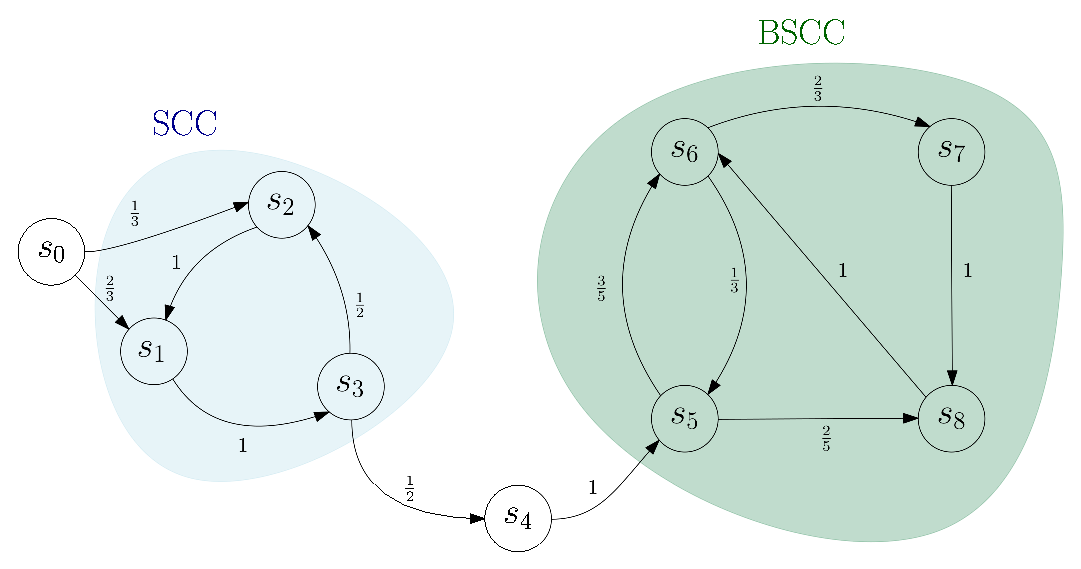
\includegraphics[width=0.7\linewidth]{resources/BSCC}
    \captionsetup{justification=centering}
    \caption{Markov chain $\mathcal{M}$ with state space composed by nine states, containing four SCCs and one BSCC}\label{bsccex}
  \end{figure}
\end{example}
\noindent We have that the subset $T = \{s_1, s_2, s_3\} \subseteq S$ is an SCC because $T$ is the largest subset containing the state $s_1$ such that all states are connected to each other.
However, $T$ is not a BSCC because the state $s_3 \in T$ is connected to $s_4$ by an edge in the underlying graph of $\mathcal{M}$ (we have $\Delta(s_3, s_4) > 0$), and $s_4$ is not connected to $T$.
Furthermore, the subset $B = \{s_5, s_6, s_7, s_8\} \subseteq S$ is a BSCC.
Indeed, $B$ is the largest subset of $S$ containing $s_5$ such that all states are connected to each other. Moreover, each state $s \in B$ verify the following assertion:
$\Delta(s, B)=1$.

\begin{theorem}[\textit{\textbf{Limit behaviour of Markov chains}}]\label{MCbehav}
Let $\mathcal{M}$ be an MC with state space $S$ and $s \in S$
be a state of $\mathcal{M}$,
\[
  \mathbb{P}_s(\{\pi \in Paths(s) \; | \; inf(\pi) \in \BSCC(\mathcal{M})\}) = 1,
\]
where $inf(\pi)$ denotes the set of states encountered infinitely often along $\pi = s_0 s_1 s_2 \dots \in Paths(s)$, i.e., $inf(\pi) = \{ s \in S \; | \; \forall n \in \mathbb{N},\, \exists m \geq n,\, s_m = s\}$.
\end{theorem}
Theorem \ref{MCbehav} means that, starting from any state of an MC, the system ends up in a BSCC with probability one, and all states of this BSCC are visited infinitely often.

\begin{corollary}[\textbf{\textit{Quantitative repeated reachability}}]
  Let $\mathcal{M}$ be a finite MC with state space $S$, $T \subseteq S$ be a subset of states of $\mathcal{M}$, and $s \in S$ be a state of $\mathcal{M}$.
  Then, we can compute the probability to encounter infinitely often $T$ as follows:
  \[
    \mathbb{P}_s(\Box \Diamond T) = \mathbb{P}_s(\Diamond U),
  \]
  where $U$ is the union of all BSCCs $B$ of $\mathcal{M}$ such that $B \cap T \neq \emptyset$. Furthermore, we can compute the probability that $T$ is persistent as follows:
  \[
    \mathbb{P}_s(\Diamond \Box T) = \mathbb{P}_s(\Diamond U),
  \]
  where $U$ is the union of all BSCCs $B$ of $\mathcal{M}$ such that $B \subseteq T$.
\end{corollary}

\begin{proof2} Let $t \in T$ be a target state.
\begin{enumerate}
\item
Let $B \in \BSCC(\mathcal{M})$ be a BSCC of $\mathcal{M}$.
In particular, assume there exists a state $t \in T$ such that $t \in B$, then $\mathbb{P}_s(\Diamond B) = \mathbb{P}_s(\{ \pi \in Paths(s) \; | \; t \in inf(\pi) \; \wedge \; inf(\pi) = B \})$. Following the definition of BSCCs, we have that $B$ is the largest subset containing $t$ such that all states of $B$ are connected to each other and such that $\forall s' \in B, \, \Delta(s', B)=1$. Then, $B$ is the only BSCC containing $t$. So,
$\mathbb{P}_s(\Diamond B) = \mathbb{P}_s(\{ \pi \in Paths(s) \; | \; t \in inf(\pi)\}) = \mathbb{P}_s(\Box \Diamond \{t\})$,
by definition of $inf(\pi)$ and $\Box\Diamond \{t\}$.
\label{B1}
%\item Furthermore, let $t \in T$, it stills to show that if $\mathbb{P}_s(\Box \Diamond \{t\}) > 0$, then we always have that there exists a BSCC $B$ such that $\mathbb{P}_s(\Diamond B)>0$, $t \in B$. By contraposition, let assume that for all BSCC $B$ such that $\mathbb{P}_s(\Diamond B) > 0$, $t \centernot\in B$.
\item
Furthermore, assume that for all BSCC $B$, $t \notin B$. As we have \[\mathbb{P}_s(\{\pi \in Paths(s)\; | \; t \notin inf(\pi), \, inf(\pi) \in \BSCC(\mathcal{M})\}) = 1,\]
we obviously have $\mathbb{P}_s(\{\pi \in Paths(s)\; | \; t \in inf(\pi)\}) = 0$, i.e., $t$ is never visited infinitely often with a positive probability, and $\mathbb{P}_s(\Box\Diamond \{t\}) = 0$.
\label{B2}
\end{enumerate}
%A consequence of Theorem \ref{MCbehav} is that
%$\mathbb{P}_s(\Diamond \bigcup_{B \in BSCC(\mathcal{M})} B)
%= 1$. Then, there exists $B \in BSCC(\mathcal{M})$ such
%that $\mathbb{P}_s(\Diamond B) > 0$. If $t \in B$, then we
%have $\mathbb{P}_s(\Box\Diamond\{t\})>0$.
By \ref{B1}, we have that if $t$ is in a BSCC $B$, then the BSCC $B$ is the only one containing $t$ and the probability to reach $B$ is equals to the probability to encounter infinitely often $t$. Furthermore, by \ref{B2}, we have that if $t$ is encountered infinitely often, then $t$ is necessarily in a BSCC. Thus,
we can generalise \ref{B1} and \ref{B2} for all states in the set $T$:
\[\mathbb{P}_s(\Box \Diamond T) = \mathbb{P}_s(\Diamond \bigcup_{B \in \BSCC(\mathcal{M}) \; | \; \exists t \in T, \, t \in B } B)\]
The second assertion can be shown in a similar way.
%\vspace{-0.1\linewidth}
\end{proof2}\\

Now, we come back on a problem addressed previously in Remark \ref{remarkS0S1}. Indeed, following an MC $\mathcal{M}$ with state space $S$ and two subsets $C, T \subseteq S$, we have presented a graph theory based solution to compute the largest subset $S_{=0}$, i.e., $\{s \in S \; | \; \mathbb{P}_s(C \U T) = 0\}$, but we have not yet presented a solution to compute the largest subset $S_{=1}$, i.e., $\{s \in S \; | \; \mathbb{P}_s(C \U T) = 1\}$.
We will see that this qualitative property can be verified thanks to the notion of BSCC.

\begin{notation}[\textit{Absorbing state}]
  Let $\mathcal{M}=(S, \Delta, w, AP, L)$ be an MC and $s \in S$ be a state of $\mathcal{M}$. We say that $s$ is absorbing iff $\Delta(s, s') = 1$.
\end{notation}

\begin{theorem}[\textbf{\textit{Almost sure reachability}}]\label{asr}
  Let $\mathcal{M}$ be a finite MC with state space $S$, $s \in S$, $T \subseteq S$ be a set of absorbing states, and the two following successors and predecessors sets:
\begin{align*}
  Succ^*(s) &= \{ s' \in S \; | \; \exists \pi = s_0s_1s_2\dots \in Paths(s) \;\; \exists k \in \mathbb{N}_0, \, s_k = s' \}, \\
  Pred^*(T) &= \{ s' \in S \; | \; \exists \pi = s_0s_1s_2\dots \in Paths(s')\; \exists k \in \mathbb{N}_0, \, s_{k} \in T \,\}.
\end{align*}
   Then , the following statements are equivalent:
  \begin{enumerate}[(a.)]
    \item $\mathbb{P}_s(\Diamond T)= 1$. \label{succ1}
    \item $Succ^*(s') \cap T \neq \emptyset, \; \forall s' \in Succ^*(s)$.\label{succ2}
    \item $s \in S \setminus Pred^*(S \setminus Pred^*(T))$. \label{succ3}
  \end{enumerate}
  In particular, \[
  \{s \in S \; | \; \mathbb{P}_s(\Diamond T) = 1\} =
  S \setminus Pred^*(S \setminus Pred^*(T))
  \]
  \begin{figure}[h]
  \centering
  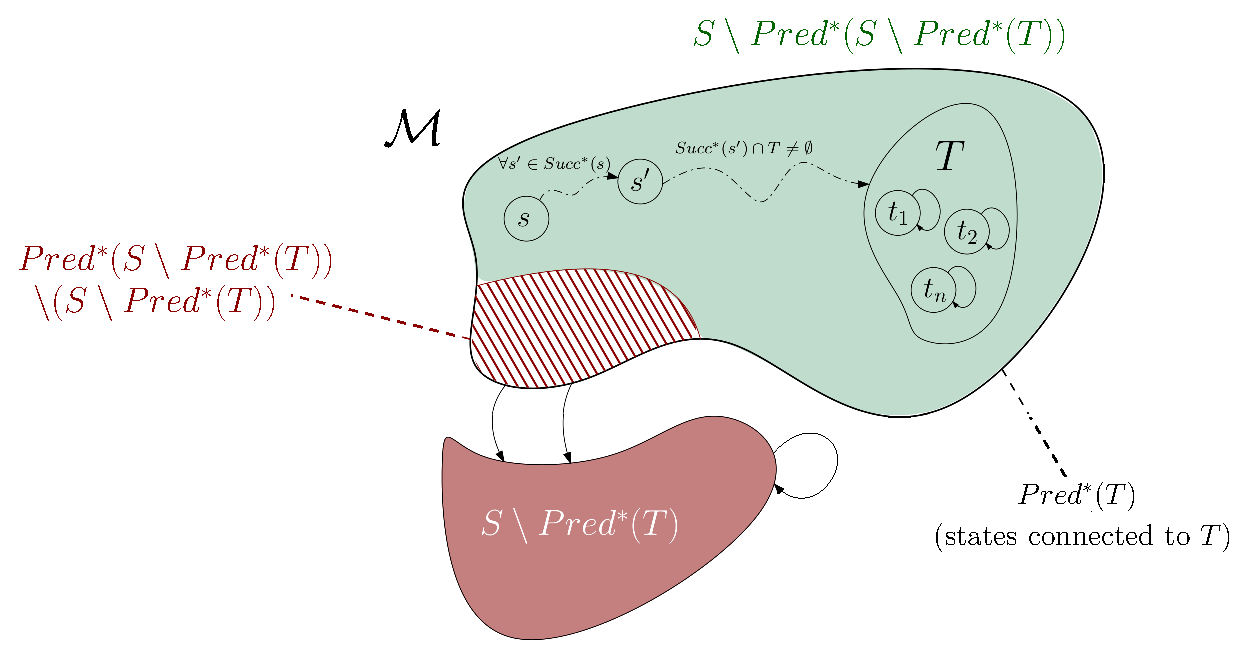
\includegraphics[width=0.93\linewidth]{resources/S2BSCC}
  \caption{Intuitive representation of the subset $S \setminus Pred^*(S \setminus Pred^*(T))$}\label{spred}
  \end{figure}
\end{theorem}
\begin{proof2}\cite{PMC}
We can easily derivate from the definitions of the sets $Succ^*$ and $Pred^*$ that \ref{succ2} and \ref{succ3} are equivalent. \\
($\neg\ref{succ2}\implies\neg\ref{succ1}$). Let $s' \in Succ^*(s)$ such that $Succ^*(s') \cap T = \emptyset$. In Figure \ref{spred}, we have that $s$ is either in the subset represented by a red tiling pattern or in the red subset, and that $s'$ is in the red subset.
The sets $Succ^*(s)$ and $Succ^*(s')$ associated with these two possible situations are depicted in Figure \ref{2sit}.
Thus, $s'$ is a successor of $s$ from which $T$ cannot be reached. Then, we have $\mathbb{P}_s(\Diamond T) \leq 1 - \mathbb{P}_s(\Diamond \{s'\}) < 1$.
%Furthermore, referring the figure
%\ref{spred}, we have that $1 - \mathbb{P}_s(\Diamond T) = \mathbb{P}_s(\Diamond (S \setminus Pred^*(T)))$.\\
\begin{figure}[H]
  \begin{minipage}{0.5\linewidth}
    \centering
    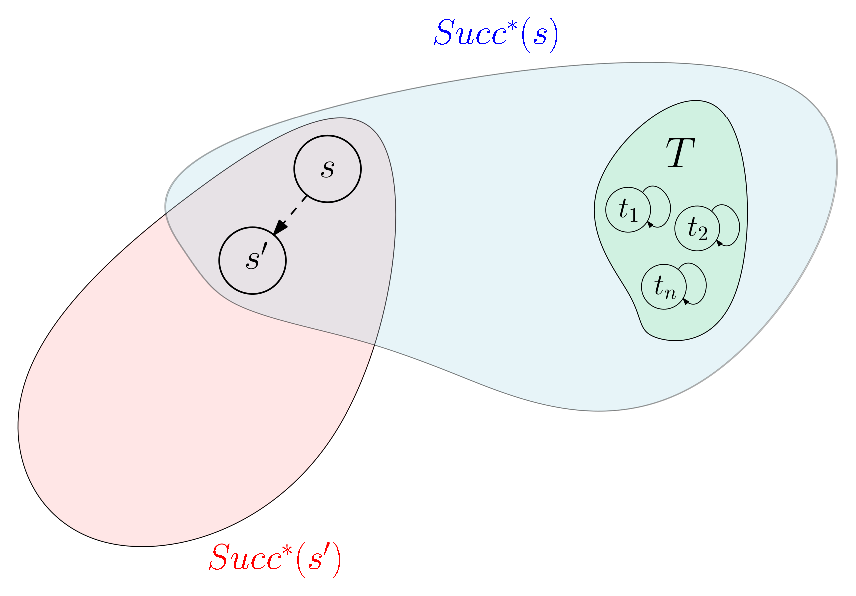
\includegraphics[width=0.8\linewidth]{resources/S3BSCC}
  \end{minipage}
  \begin{minipage}{0.5\linewidth}
    \centering
    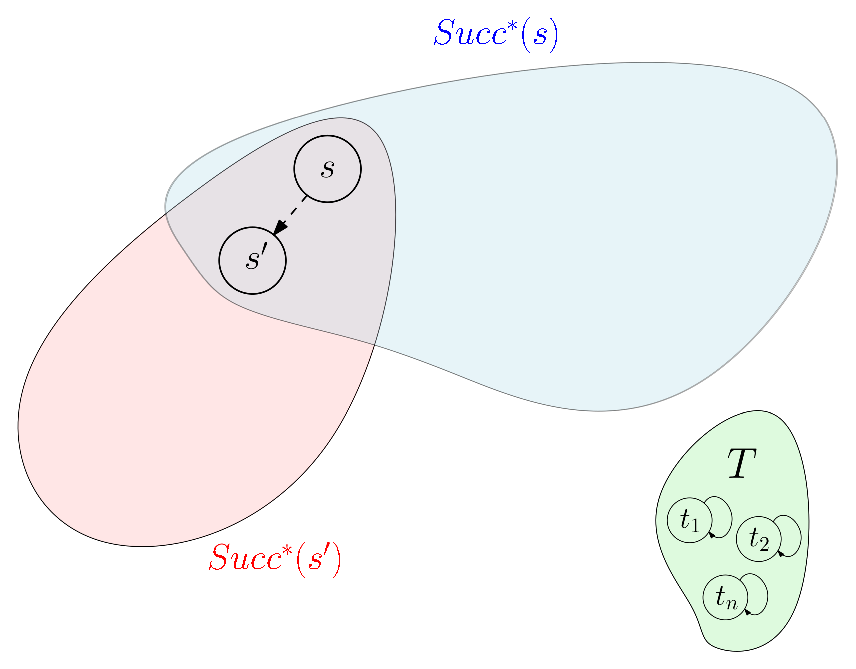
\includegraphics[width=0.8\linewidth]{resources/S4BSCC}
  \end{minipage}
  \captionsetup{justification=centering}
  \caption{Intuitive representation of the sets $Succ^*(s)$ and $Succ^*(s')$ in the two possible situations}
  \label{2sit}
\end{figure}
\noindent($\ref{succ2} \implies \ref{succ1}$). Assume that $Succ^*(s') \cap T \neq \emptyset$, for any successor $s'$ of $s$. By Theorem \ref{MCbehav}, we reach a BSCC from $s$ with probability one. Since each state in $t \in T$ is absorbing, each BSCC $B$ of $\mathcal{M}$ consists in $B = \{t\}$ or it satisfies $T \cap B = \emptyset$. We will show that the latter case can not occur from $s$.
Consider $T \cap B = \emptyset$ for some BSCC $B$.
As $B$ is a BSCC, $Succ^*(u)\cap T = \emptyset$, for each $u \in B$.
However, as $T$ is reachable for any $s' \in Succ^*(s)$, there is no BSCC with $T \cap B = \emptyset$ that is reachable from $s$. So, we almost surely have a state in $T$ that will be reached from the state $s$.
\end{proof2}
\\

Theorem \ref{asr} allows to compute the largest subset $S_{=1} = \{s \in S \; | \; \mathbb{P}_s(\Diamond T) = 1 \}$ for any finite MC with state space $S$ and for any $T \subseteq S$ as follows:
%Indeed, we begin by make all states in $T$ absorbing. This allows to apply Theorem \ref{asr}.
%Then, we can compute all states connected
\begin{algorithm}[H]
\caption{Almost sure reachability}\label{almost-sure-algo}
\begin{algorithmic}[1]
  \REQUIRE a finite Markov chain $\mathcal{M}$ with state space $S$, a transition function $\Delta$, and a set of target states $T \subseteq S$.
  \ENSURE the set $\{ s \in S \; | \; \mathbb{P}_s(\Diamond T) = 1\}$.
  \item[]
  \STATE $\Delta_T \leftarrow \lambda (s, s'):\, \begin{cases}
    1 &\text{if } s = s' \text{ and } s \in T\\
    \Delta(s, s') &\text{else}
  \end{cases}$
  \STATE $\mathcal{M}_T \leftarrow (S, \Delta_T)$
  \COMMENT{make all states of $T$ absorbing, yielding a new MC $\mathcal{M}_T$}
  \STATE $Pre^*(T) \leftarrow \mathsf{backward\_search}(G^{\mathcal{M}_T}, T)$
  \COMMENT{compute the set of states connected to $T$}
  \STATE $Pre^*(S \setminus Pre^*(T)) \leftarrow \mathsf{backward\_search}(G^{\mathcal{M}_T}, S \setminus Pre^*(T))$
  \RETURN $S \setminus Pre^*(S \setminus Pre^*(T))$
\end{algorithmic}
\end{algorithm}
\noindent where the notation $\lambda x:y$ is a lambda calculus based notation that gives the lambda calculus expression $\lambda x.y \equiv x \mapsto y$, $G^\mathcal{M}$ denotes the underlying graph of $\mathcal{M}$ and the $\mathsf{backward\_search}$ algorithm
, for inputs $G^{\mathcal{M}_T}$ and $T$, explores $G^{\mathcal{M}_T}$ from the set $T$: it starts by marking all states of $T$, and then iteratively marks all unmarked predecessors of marked states (\textit{backward breadth-first search}). All marked states are thus connected to $T$. An alternative recursive version of this algorithm exists (\textit{backward depth-first search}).
The time complexity of this algorithm is in $\mathcal{O}(|\mathcal{M}_T|)$.

\begin{corollary}[\textbf{\textit{Qualitative constrained reachability}}]\label{qualitative-const-reach} Let $\mathcal{M}$ be an MC with state space $S$ and $C, T \subseteq S$, the sets
\[
  S_{=0} = \{ s \in S \; | \; \mathbb{P}_s (C \U T) = 0 \} \text{ and } S_{=1} = \{ s \in S \; | \; \mathbb{P}_s (C \U T ) = 1 \}
  \]
  can be computed in time $\mathcal{O}(|\mathcal{M}|)$.
\end{corollary}
\begin{proof2}\cite{PMC}
\begin{enumerate}
  \item We can determine $S_{=0}=\{s \in S \; | \; \mathbb{P}_s(C \U T)=0\}$ by computing the complement of the set $\{s \in S \; | \; \exists \pi \in Paths(\pi), \, \pi \models C \U T \}$ (cf. Lemma \ref{S0graph}).
  \item A linear-time algorithm for the computation of $S_{=1}=\{ s\in S \; | \; \mathbb{P}_s(C \U T) = 1 \}$ can be obtained by a reduction to the reachability problem to $T$ in a slightly modified MC. The idea is the following: we make all states of $T$ absorbing (to take advantage of Theorem \ref{asr}) and do the same for all states in $S \setminus (C \cup T)$.
  The probability transition function of this modified MC $\mathcal{M}'$ is
  defined as follows:
  \[
    \Delta'(s, s') = \begin{cases}
      1 & \text{if } s=s' \text{ and } s'\in T \cup (S \setminus(C \cup T)),\\
      0 & \text{if } s \neq s' \text{ and } s \in T \cup (S \setminus (C \cup T)),\, \text{and}\\
      \Delta(s, s') & \text{otherwise}.
    \end{cases}
  \]
  Thus, we have:
  \begin{itemize}
    \item $\mathbb{P}_s^\mathcal{M}(C \U T) = \mathbb{P}_s^\mathcal{M'}(\Diamond T)$ for all states $s \in C \setminus T$,
    \item $\mathbb{P}_s^\mathcal{M}(C \U T) = \mathbb{P}_s^{\mathcal{M}'}(\Diamond T) = 1$
    for all states $s \in T$, and
    \item $\mathbb{P}_s^\mathcal{M}(C \U T)= \mathbb{P}_s^{\mathcal{M}'}(\Diamond T) = 0$ for all states $s \in S \setminus (C \cup T)$.
  \end{itemize}
  Doing this reduction, we can apply Theorem  \ref{asr} to compute the largest set $S_{=1}$ with Algorithm \ref{almost-sure-algo}.
\end{enumerate}
\end{proof2}\\

Thus, check if each temporal event presented in this section holds with probability one or zero can be done through simple graph theory algorithms in $\mathcal{O}(|\mathcal{M}|)$, without referring to probabilities of transitions.

\subsection{Temporal events in Markov decision processes}
We present in this subsection a way to deal with temporal events in MDPs and furthermore compute their probability.
In the first chapter, we have approached a method allowing to compute the optimal strategy $\sigma$ for the \SR{} problem, i.e., compute the strategy $\sigma$ following an MDP $\mathcal{M}$ with state space $S$, a state $s \in S$, and a subset of target states $T$, such that $\mathbb{P}_s^\sigma(\Diamond T) = \max_{\sigma} \mathbb{P}^{\sigma}_s(\Diamond T) = \mathbb{P}^{\max}_s(\Diamond T)$.
We have seen that this can be done in polynomial time in the size of $\mathcal{M}$, through a linear program (cf. Theorem \ref{thm-sr} and Appendix \ref{app-sr}).
We can generalise this computation of optimal strategy for the constrained reachability events. To this purpose, we need to address the equation system from which the linear program used to compute this strategy is derived (cf. Appendix \ref{app-sr}).

\begin{definition}[\textbf{Connectivity to a subset of target states}]\label{connectivity-def}
  Let $\mathcal{M}$ be an MDP with state space $S$ , $s \in S$, and $T \subseteq S$.
  The state $s$ is said to be \textit{connected to $T$} if and only if there exists a path $\pi = s_0\xrightarrow{\alpha_1}s_1\xrightarrow{\alpha_2}s_2 \xrightarrow{\alpha_3} \dots \in Paths(s)$ such that there exists a state $s_k \in T$ for $k \in \mathbb{N}$.
\end{definition}

\begin{theorem}[\textbf{\textit{Bellman's equation system for optimal reachability probabilities}}] \label{bellman1}
  Let $\mathcal{M}$ be an MDP with state space $S$ and with a probability transition function $\Delta$, $s \in S$ be a state of $\mathcal{M}$ and $T \subseteq S$ be a subset of target states. The vector $(x_s)_{s \in S}$ with $x_s = \mathbb{P}_s^{\max}(\Diamond T)$ yields the unique solution of the following equation system: let the subset $S_{=1} \subseteq S$ be a subset of states such that $T \subseteq S_{=1} \subseteq \{s \in S \; | \; \mathbb{P}^{\max}_s(\Diamond T) = 1 \}$,
  \begin{enumerate}[(1.)]
    \item if $s \in S_{=1}$, then $x_s=1$,
    \label{bellman-cond1}
    \item else if $s$ is not connected to $T$, then $x_s=0$,
    \label{bellman-cond2}
    \item else,
    \[ x_s = \max_{\alpha \in A(s)} \sum_{s' \in Succ(s, \alpha)} \Delta(s, \alpha, s') \cdot x_{s'}. \]
    \label{bellman-cond3}
  \end{enumerate}
\end{theorem}
This theorem suggests an iterative approximation technique, called \textit{value iteration}, to compute the values $x_s=\mathbb{P}^{\max}_s(\Diamond T)$ for $s \in S$.
First, we assume $x_s^{(n)}$ being equal to $x_s$ for all $n \in \mathbb{N}$, for each state $s \in S$ verifying conditions \ref{bellman-cond1} and \ref{bellman-cond2} determined by a backward reachability analysis of the underlying graph of $\mathcal{M}$. For other states $s$, we have
\[x_s = \lim_{n \rightarrow \infty} x_s^{(n)}\]
where
\[x_s^{(0)} = 0 \quad \text{and} \quad x_s^{(n+1)} = \max_{\alpha \in A(s)} \sum_{s' \in Succ(s, \alpha)} \Delta(s, \alpha, s') \cdot x_{s'}^{(n)}. \]
This yields $x_s^{(n)} \leq x_s^{(n+1)}$ for any $n \in \mathbb{N}$, and the values of $\mathbb{P}^{\max}_s(\Diamond T)$ can be approximated by iteratively computing vectors $x_s^{(n+1)}$
with vectors $x_s^{(n)}$ for all states $s \in S$ until $\max_{s \in S} |x_s^{(n+1)} - x_s^{(n)}| < \varepsilon$ for a small threshold value $\varepsilon > 0$.
\begin{theorem}[\textbf{\textit{Value iteration for step-bounded reachability}}] \label{theo-value-it}
  Let $\mathcal{M}$ be an MDP with state space $S$ and with a probability transition function $\Delta$, and $T \subseteq S$ be a subset of target states. The value iteration approach can be used to compute the maximal probabilities for the event $\Diamond^{\leq n}T$.
  Indeed, the vector $(x_s)^{(n)}_{s \in S}$ with $x_s^{(n)} = \mathbb{P}^{\max}_s(\Diamond^{\leq n} T)$ yields the unique solution of the following equation system:
  \begin{itemize}
    \item if $s \in T$, then $x_s^{(n)}=1$ for all $n \in \mathbb{N}$,
    \item else if $s$ is not connected to $T$, then $x_s^{(n)}=0$
    for all $n \in \mathbb{N}$,
    \item else, $x_s^{(0)} = 0$ and
    \[ x_s^{(n+1)} = \max_{\alpha \in A(s)} \sum_{s' \in Succ(s, \alpha)} \Delta(s, \alpha, s') \cdot x_{s'}^{(n)}. \]
  \end{itemize}
\end{theorem}
  According to the equation system defined in Theorem \ref{theo-value-it}, we can build a finite memory strategy $\sigma = (Q, \sigma_{act}, \delta, \delta_0)$ such that $\mathbb{P}^\sigma_s(\Diamond^{\leq n}\, T) = \mathbb{P}^{\max}_s(\Diamond^{\leq n}\, T)$ for $s \in S$ and $n \in \mathbb{N}$:
  assume that modes of $Q$ range from $0$ to $n$ such that $\delta_0(s) = m_0$ and $\delta(m_i, s) = m_{\min\{i+1, n\}}$ for all $s \in S$ and $i \in \{0, \dots, n\}$. Then, we define $\sigma_{act}$ as follows:
  \[
    \sigma_{act}(m_i, s) =
    \begin{cases}
      \alpha \text{ such that } \alpha \in A(s) &\text{if }i = n,\\
      \arg \max_{\alpha \in A(s)} \sum_{s' \in Succ(s, \alpha)} \Delta(s, \alpha, s') \cdot x_{s'}^{(i)}
      & \text{else.}
    \end{cases}
  \]
  Intuitively, $\sigma$ is initialised in mode $m_0$, and when the strategy is in mode $m_i$ for $i \in \{0, \dots, n-1\}$,
  it chooses the action that maximises $\sum_{s' \in Succ(s, \alpha)} \Delta(s, \alpha, s') \cdot x_{s'}^{(i)}$ and then go to the next mode $m_{i+1}$. When the strategy enters in mode $m_n$, it stays inside it forever and always chooses an arbitrary enabled action. \\

\begin{theorem}[\textbf{\textit{Strategy for constrained reachability}}] \label{cut-strategy}
  Let $\mathcal{M}$ be an MDP with state space $S$, $s \in S$, $C, T \subseteq S$, and $n \in \mathbb{N}$.
  We can build a strategy $\sigma$ and a strategy $\sigma'$ respectively satisfying $\mathbb{P}_s^\sigma (C \U T) = \max_{\sigma} \mathbb{P}_s^\sigma(C \U T)$ and
$\mathbb{P}_s^{\sigma'} (C \U^{\leq n}\, T) = \max_{\sigma} \mathbb{P}_s^\sigma(C \U^{\leq n}\, T)$
in polynomial time in the size of $\mathcal{M}$.
\end{theorem}
\begin{proof2}
We can compute $\mathbb{P}_s^{\max}(C \U T)$ (or $\mathbb{P}_s^{\max}(C \U^{\leq n} \, T)$) for any state $s \in S$ of the system by reduction to the reachability to $T$ as follows:
we make all states $s^* \in S \setminus (C \cup T)$ absorbing, i.e., we replace all enabled actions in $A(s^*)$
by a unique action $\alpha_{s^*}$ such that $\Delta(s^*, \alpha_{s^*}, s^*) = 1$.
Then, we build a strategy $\sigma$ such that $\mathbb{P}^{\sigma}_s(\Diamond T) = \mathbb{P}^{\max}_s(\Diamond T)$ (or $\mathbb{P}^{\sigma}_s(\Diamond T) = \mathbb{P}^{\max}_s(\Diamond^{\leq n}\, T)$) in this modified MDP.
For $\mathbb{P}_s^{\max}(\Diamond T)$, this strategy corresponds to the optimal strategy built for the \SR{} problem for the state $s$, the subset of target states $T$, and an arbitrary probability threshold (cf. Appendix \ref{app-sr} for more details on the computation of this maximum probability).

\end{proof2}
$ $\\

In order to optimise computations and the size of the LP defined to determine
$\mathbb{P}_s^{\max}(\Diamond T)$ for all $s \in S$,
it is possible to efficiently compute the largest set $S_{=1} = \{s \in S \; | \; \mathbb{P}_s^{\max}(\Diamond T) = 1 \}$.

\begin{theorem}[\textbf{\textit{Qualitative reachability in MDPs}}]
  Let $\mathcal{M}$ be an MDP with state space $S$, and $T \subseteq S$.
  The set
  \[
    S_{=1} = \{ s \in S \; | \; \mathbb{P}^{\max}_s(\Diamond T) = 1 \}
  \]
  can be computed in time $\mathcal{O}(|\mathcal{M}|^2)$.
\end{theorem}
The set of states almost surely reaching $T$ under the control of an optimal strategy can be computed with Algorithm \ref{prMax1}.
\begin{algorithm}[H]
\caption{Build the largest subset $S_{=1}$}
\label{prMax1}
\begin{algorithmic}[1]
\REQUIRE{
		$\mathcal{M} = (S, A, \Delta, w, AP, L)$, an MDP, and
		$T \subseteq S$, a subset of target states.
	}
\ENSURE{
	The set of states $s$ of $\mathcal{M}$ for which
		$\mathbb{P}_{s}^{\max} (\Diamond T)= 1$.
}
\STATE $U \gets \{ s \in S \; | \; s \text{ is not connected
%\footnote{cf. Definition \ref{connectivity-def}
to } T\}$ \label{pr1-bad-states}
\COMMENT{$U$ is the set of ``bad states''}
\WHILE{$U \neq \emptyset$} \label{under-loop}
	\STATE $R \gets U$
	\WHILE{$R \neq \emptyset$}
		\STATE Let $u \in R$
		\COMMENT{let $u$ be a bad state}
		\STATE $R \gets R \setminus \{u \}$
		\COMMENT{mark $u$ as visited}
		\FORALL{$(s, \alpha) \in Pred(u)$ such that $s \not\in U \cup T$} \label{pr1-remove-1}
			\STATE remove $\alpha$ from $A(s)$
			\COMMENT{remove all ingoing edges of $u$} \label{pr1-remove-2}
			\IF{$A(s) = \emptyset$} \label{pr1-remove-3}
				\STATE $R \gets R \cup \{s\}$
				\COMMENT{\scriptsize for any enabled action, $s$ is always connected to a bad state}
				\STATE $U \gets U \cup \{s\}$ \label{pr1-remove-4}
				\COMMENT{thus, $s$ is marked as bad state}
			\ENDIF
		\ENDFOR
		\STATE remove $u$ and its outgoing edges in $\mathcal{M}$
	\ENDWHILE
	\STATE $U \gets \{ s \in S \setminus U \; | \; s \text{ is not connected to } T \}$ \label{pr1-unconnected}
	\COMMENT{\scriptsize update the set of bad states}
\ENDWHILE
\RETURN the remaining states
\end{algorithmic}
\end{algorithm}
In order to compute this set of states, we consider $\mathcal{M}$ as being a directed graph.
This directed graph is a refinement of its underlying graph, where the successors of any vertex $s \in S$ are new dummy vertices being the pairs $(s, \alpha)$, with $\alpha \in A(s)$.
The outgoing edges of these dummy vertices $(s, \alpha)$ are $\alpha$-successors of $s$.
The key idea is looking at all ``bad states'', unconnected to the set of target states $T$ (cf. line \ref{pr1-bad-states}), and iteratively remove all dummy vertices of this modified graph having an outgoing edge to these bad states (cf. lines \ref{pr1-remove-1} and \ref{pr1-remove-2}).
That is, we remove these dummy vertices as well as their ingoing and outgoing edges.
If a vertex representing a state $s$ has no more outgoing edge to a dummy state, then whatever the enabled action chosen in the MDP by any strategy at state $s$, the system could in the worst case never reach $T$ (i.e., the system do not almost surely reach $T$ from $s$).
In that case, such a state is tagged as being a bad state (cf. lines \ref{pr1-remove-3} and \ref{pr1-remove-4}), and we repeat the operation until all the bad states have been considered.
After that, we compute the set of states unconnected to $T$ again and mark them as bad states (cf. line \ref{pr1-unconnected}).
Indeed, deleting dummy states could leave some bad states in the graph (e.g., an SCC unconnected to $T$ could remain).
We repeat all the operations since the beginning for these new bad states until no more bad states are found in the last step of the algorithm.
The states unmarked as bad states are finally returned.\\

This algorithm is exact (cf. \cite{PMC} for the correctness proof) and is quadratic in the size of $\mathcal{M}$.
Indeed, this can be seen easily: the maximal number of iterations of the outermost loop (cf. line \ref{under-loop}) is $|S|$ (a state can be marked as bad at most once).
Then, in each iteration of this outermost loop, the set of states unconnected to $T$ is computed in time $\mathcal{O}(|\mathcal{M}|)$ by backward search from $T$ in the modified directed graph.
Finally, the rest of operations cause in worst case time in $\mathcal{O}(|\mathcal{M}|)$, since states can be marked and dummy states can be removed at most once.

\section{Probabilistic computation tree logic}\label{pctl-section}
\textit{Probabilistic computation tree logic} (PCTL, for short) is a \textit{branching-time temporal logic}.
This logic allows to verify probabilistic systems via an
%probabilistic
execution tree, actually named \textit{computation tree}.
In this section, we describe this logic for Markov chains. \\

For a given system, the computation tree consists of an infinite unfolding of this system starting from a given state (i.e., the root of the tree), considering
all branching possibilities.
%Thus, it is actually an MC with an infinite tree as underlying graph.
The key ideas behind this tree are that
each node of the tree corresponds to a state of the system, and
each prefix of the tree corresponds to a finite path of the system starting from the root of the tree.
%and finally that
%each branch of a node leads to a possible future of this node.
Moreover, each branch passing by a node of the tree corresponds to a path of the system having the prefix leading the root to the node in the tree in its set of prefixes.
So, in Markov chains context, this tree is highly linked to cylinder sets:  %Possible futures of a node actually correspond to paths of the cylinder set formed by the prefix leading the root to the node in the tree.
all branches of the tree passing by a node corresponds to the cylinder set spanned with the prefix leading the root to the node in the tree.

\begin{example}[\textit{Computation tree of an MC}]
Let $\mathcal{M}$ be the MC with state space $S$ and labelling function $L$ of Figure \ref{ct1}. The computation tree of $\mathcal{M}$ starting from the state $s_0$ is
given in Figure \ref{ct2}.
We clearly see that any branch passing by a node $s^*$ in this tree actually corresponds to a path $\pi = s_0 \dots s_k {\, \dots} \in Cyl(s_0 \dots s_k)$ such that $s_k=s^*$.
For example,
%$s_1$ is a possible future of the node $s_0$ (for which the prefix is $s_0s_0$ in the tree) because the path $\pi = s_0s_0s_0(s_1s_2)^\omega$ is in $Cyl(s_0s_0)$.
the path $\pi = s_0s_0(s_1s_2)^\omega \in Cyl(s_0s_0)$ is a branch of the tree passing by the node $s_0$ having $s_0s_0$ as prefix.
\begin{figure}[h]
  \begin{minipage}{0.4\linewidth}
    \centering
    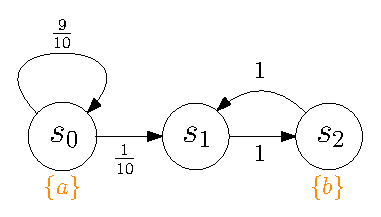
\includegraphics[width=0.8\linewidth]{resources/CLT_unfolding_1}
    \captionsetup{justification=centering}
    \captionof{figure}{MC $\mathcal{M}$ with $3$ states, $s_0, s_1$ and $s_2$, and $2$ atomic propositions, $a$ and $b$}\label{ct1}
  \end{minipage}
  \begin{minipage}{0.6\linewidth}
    \centering
    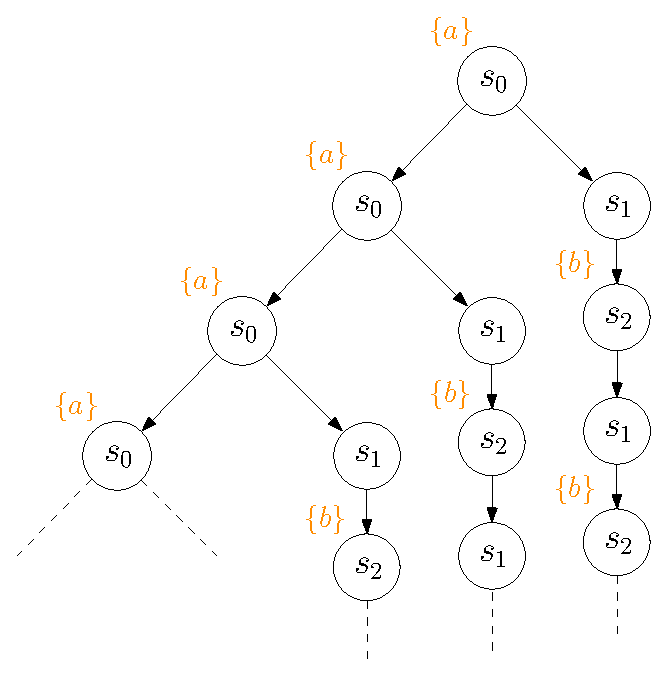
\includegraphics[width=0.8\linewidth]{resources/CLT_unfolding_2}
    \captionsetup{justification=centering}
    \captionof{figure}{Computation tree of $\mathcal{M}$ starting from $s_0$}\label{ct2}
  \end{minipage}
\end{figure}
We will see that it is possible to express formulae in PCTL describing states properties of the system like the following one:
\begin{center}
``\textit{Do all executions starting from the state $s_0$ always eventually reach $b$ with a nonzero probability ?}''
\end{center}
Model checking algorithms of PCTL will answer \textit{yes} to this question.
Intuitively, if we refer to the computation tree,
%we see that it is possible to reach a node labeled with $b$,
%from any node of the tree,
%via a path from this node that has a nonzero probability.
%we see that it is possible to reach a node labelled with $b$ from any node of the tree and, each cylinder set
%for which the prefix leads the root to any node has a nonzero probability:
we see that a node labelled with $b$ appears in the \textit{future} of any node $s^*$ in the tree: if there exists an index $n$ for each path $\pi = s'_0 s'_1 s'_2 \dots s'_n {\,\dots} \in Cyl(s'_0 \dots s'_k)$, where $s'_0 \dots s'_k$ is the prefix that leads the root to the node $s^* = s'_k$ in the tree, such that $k <n$ and $s'_n$ is labelled with $b$, then the property is verified. This is true for all paths,  except for the path $s_0^\omega$ (corresponding to the left path in the computation tree).
Since this path has a zero probability, we have that this property is verified with a probability one from the state $s_0$.
We will see in this chapter how to verify formally each property of this type by referring to Section \ref{tempevent}.
Indeed, for this example, the question can be reformulated as follows: $\mathbb{P}_{s_0}(\Box\Diamond \{ s \in S \; | \; b \in L(s)\}) > 0$.

%let $\hat{\pi} = s'_0 \dots s'_n$ be a finite path of $\mathcal{M}$, starting from the state $s_0$ of $\mathcal{M}$ and referring to a finite path starting from the root of the tree. If there exists an index $k$, such that $1 \leq k \leq n$ and $s'_k = s_1$, then $\mathbb{P}_{s_0}(Cyl(s'_0 \dots s'_k \dots s'_n)) = \prod_{i=0}^{k-1} \Delta(s'_i, s'_{i+1}) \cdot 1^\omega = \frac{1}{10}^{k-1}$.
%Else, $\hat{\pi} = s_0^{n+1}$ and $\mathbb{P}_{s_0}(Cyl(s_0^{n+1})) = \frac{1}{10}^n$.
%Furthermore, all executions starting from $s_0$ has a probability one to always eventually reach a state labeled with $b$: the only path starting from $s_0$ that does not allow it is the path $s_0^\omega$ (corresponding to the left path in the computation tree) and has a zero probability.
\end{example}

\subsection*{Syntax and semantic}
PCTL has a two stages syntax where PCTL formulae are classified into state and path formulae. Intuitively, \textit{state formulae} are assertions about atomic propositions in a state $s$ and about probabilities over their branching structure, i.e., probabilities of \textit{path formulae} starting from $s$. Actually, a path formula imposes conditions on a set of paths and this path formula is quantified
by probability bounds.

\begin{definition}[\textbf{Syntax of PCTL}]
Let $AP$ be a set of atomic propositions,
\begin{itemize}
  \item PCTL \textit{state formulae} over $AP$ are formed according to the following grammar:
  \[
    \Phi ::= true \;\; | \;\; a \;\; | \;\; \Phi_1 \wedge \Phi_2 \;\; | \;\; \neg \Phi \;\; | \;\; \mathcal{P}_J(\phi)
  \]
  where $a \in AP$ is an atomic proposition, $J \subseteq [0, 1] \cap \mathbb{Q}$ is an interval with rational bounds and $\phi$ is a path formula.
  \item PCTL \textit{path formulae} over $AP$ are formed according to the following grammar:
  \[
  \phi ::= \bigcirc \Phi \;\; | \;\; \Phi_1 \U \Phi_2 \;\; | \;\; \Phi_1 \U^{\leq n} \Phi_2
  \]
  where $\Phi$, $\Phi_1$ and $\Phi_2$ are state formulae and $n \in \mathbb{N}$.
\end{itemize}
\end{definition}
Intuitively, $\mathcal{P}_J(\phi)$ specifies that the probability of paths satisfying the path formula $\phi$ must be in the interval $J$. A path formula is formed by temporal operators, like $\bigcirc$ and $\U$, with $\U^{\leq n}$ being $\U$ bounded by a maximum number of steps.  There exist some other linear temporal operators, dealing with paths of the system (cf. Figure \ref{ltl}). These operators can be derived from the PCTL grammar:
let $J \in [0, 1]$ be an interval, $\Phi$ be a state formula and $n \in \mathbb{N}$ be a number of steps,

\makeatletter
\newcommand*\bigcdot{\mathpalette\bigcdot@{.5}}
\newcommand*\bigcdot@[2]{\mathbin{\vcenter{\hbox{\scalebox{#2}{$\m@th#1\bullet$}}}}}

\makeatother
\begin{flalign}
  &\bigcdot \; \mathcal{P}_J(\Diamond \Phi) \equiv \mathcal{P}_J(true \U \Phi) \tag{\textit{eventually} probability} \\
  &\bigcdot \; \mathcal{P}_J(\Diamond^{\leq n} \Phi) \equiv \mathcal{P}_J(true \U^{\leq n} \Phi) \tag{\textit{bounded enventually} probability} \\
  &\bigcdot \; \mathcal{P}_J(\Box \Phi) \equiv
    \neg \mathcal{P}_J(\Diamond \neg \Phi)
    \tag{\textit{always} probability} \\
  &\bigcdot \; \mathcal{P}_J(\Box^{\leq n} \Phi) \equiv
    \neg \mathcal{P}_J(\Diamond^{\leq n} \neg \Phi)
    \tag{\textit{bounded always} probability}
\end{flalign}

\begin{figure}[h]
  \centering
  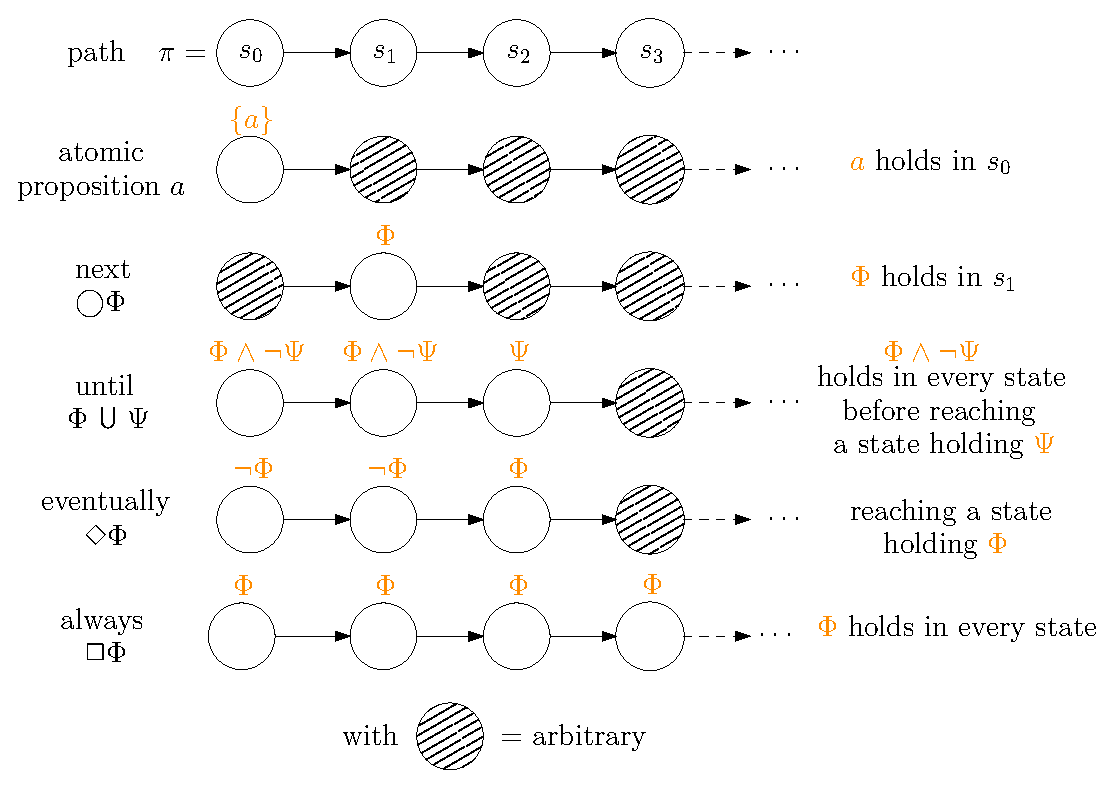
\includegraphics[width=0.85\linewidth]{resources/LTL}
  \caption{Intuitive semantic of linear temporal operators}\label{ltl}
\end{figure}

%Let $\mathcal{M}$ be an MC with state space $S$, $s \in S$, and $\pi = s_0$

\begin{definition}[\textbf{Semantic of PCTL}]
  Let $\mathcal{M} = (S, \Delta, w, AP, L)$ be an MC, $s \in S$, $\Phi, \Psi$ be PCTL state formulae over $AP$, and $\phi$ be a PCTL path formula over $AP$,
  \begin{flalign*}
  \intertext{$s \models \Phi$ iff the state formula $\Phi$ holds in the state $s$, i.e.,}
    &\bigcdot\; s \models true, &&&\\
    &\bigcdot\; s \models a &\text{ iff }& a \text{ is a label of $s$, i.e., } a \in L(s),&\\
    &\bigcdot\; s \models \Phi \wedge \Psi &\text{ iff }& s \models \Phi \text{ and } s \models \Psi ,&\\
    &\bigcdot\; s \models \neg \Phi &\text{ iff }& s \not\models \Phi, &\\
    &\bigcdot\; s \models \mathcal{P}_J(\phi) &\text{ iff }& \mathbb{P}_s(\{ \pi \in Paths(s) \; | \; \pi \models \phi \}) \in J.& \\
  \intertext{Following a path $\pi = s_0s_1s_2\dots \in Paths(s)$, $\pi \models \phi$ iff $\pi$ satisfies the path formula $\phi$, i.e., }
  &\bigcdot\;\pi \models \bigcirc\, \Phi&\text{ iff }&s_1 \models \Phi,&\\
  &\bigcdot\;\pi \models \Phi \U \Psi &\text{ iff }& \exists j \in \mathbb{N},\, s_j \models \Psi
    \text{ and } \forall i \in \mathbb{N}, \, i < j, \, s_i \models \Phi,&\\
  &\bigcdot\;\pi \models \Phi \U^{\leq n} \Psi &\text{ iff }& \exists j \in \mathbb{N}, \, j \leq n ,\, s_j \models \Psi
    \text{ and } \forall i \in \mathbb{N}, \,i < j, \, s_i \models \Phi.&\\
  \intertext{Additionally,}
  &\bigcdot\; \pi \models \Diamond \Phi&\text{ iff }& \exists j \in \mathbb{N}, \, s_j \models \Phi,&\\
  &\bigcdot\; \pi \models \Box \Phi&\text{ iff }& \forall j \in \mathbb{N}, \, s_j \models \Phi.&
  \end{flalign*}
\end{definition}
%\begin{remark}[\textit{Measurability of path formulae}]
%Since $\mathcal{P}_J(\phi)$ refers to probabilities, $\neg \mathcal{P}_J(\phi) = \mathcal{P}_{J'}(\phi)$ for any path formula $\phi$, with $J'=[0, 1] \setminus J$. Then,
The event $\{ \pi \in Paths(s) \; | \; \pi \models \phi\}$ must be measurable to verify that $\mathcal{P}_J(\phi)$ holds in any state.
In fact, these events can be formed through countable unions of cylinder sets, ensuring their measurability.
%This follows from the following theorem.
%\end{remark}

\begin{theorem}[\textit{\textbf{Measurability of PCTL path formula events}}]
  Let $\mathcal{M}$ be an MDP with state space $S$, $s \in S$ be a state of $\mathcal{M}$ and $\phi$ be a PCTL path formula, the set $\{ \pi \in Paths(s) \; | \; \pi \models \phi \}$ is a measurable event.
\end{theorem}

\begin{proof2}
Let $Paths(s, \phi) = \{ \pi \in Paths(s) \; | \; \pi \models \phi \}$.
\begin{enumerate}
  \item If $\phi = \bigcirc \Phi$, then $Paths(s, \phi)$ agrees with the union of the cylinders sets $Cyl(ss')$, where $s' \in Succ(s)$ and $s' \models \Phi$.
  \item Else, if $\phi = \Phi_1 \U \Phi_2$, then the definition of
  $\pi \models \phi$ for any $\pi \in Paths(s)$ agrees with the definition of
  $\pi \models Sat(\Phi_1) \U Sat(\Phi_2)$.
  Thus, $Paths(s, \phi) = Sat(\Phi_1) \U Sat(\Phi_2)$.
  \item Else, if $\phi = \Phi_1 \U^{\leq n}\Phi_2$ for any $n \in \mathbb{N}$, then the definition of
  $\pi \models \phi$ for any $\pi \in Paths(s)$ agrees with the definition of
  $\pi \models Sat(\Phi_1) \U^{\leq n} Sat(\Phi_2)$.
  Thus, $Paths(s, \phi) = Sat(\Phi_1) \U^{\leq n} Sat(\Phi_2)$.
\end{enumerate}
As countable union of cylinder sets and constrained reachability events are measurable (cf. Lemma \ref{cut-lemma}), $Paths(s, \phi)$ is measurable, for any path formula $\phi$.

\end{proof2}
$ $\\
\begin{remark}[\textit{Probabilistic satisfiability of path formulae}] $ $\\[-1.5em]
%Let $\mathcal{M}$ be the MC of Figure \ref{pctlctl}.
% \begin{figure}[h]
%   \centering
%   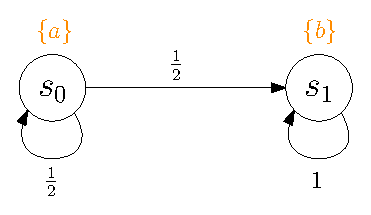
\includegraphics[width=0.25\linewidth]{resources/PCTL_CTL}
%   \captionsetup{justification=centering}
%   \caption{MC $\mathcal{M}$ with $2$ states, $s_0$ and $s_1$, and $2$ atomic propositions, $a$ and $b$}\label{pctlctl}
% \end{figure}
\begin{itemize}
% \item Let assume that there exists a path $\pi \in Paths(s_0)$ starting from $s_0$ in $\mathcal{M}$ such that $\pi \not \models \phi$, for any PCTL path formula $\phi$. That does not mean that $s_0 \models \mathcal{P}_{<1}(\phi)$: take $\pi=s_0^\omega$ and $\phi = \Diamond b$, we have that $s_0^\omega \not \models \Diamond b$ and $\mathbb{P}_s(\Diamond \{s_1\}) = 1$.
% Then $s_0 \models \mathcal{P}_{=1}(\Diamond b)$.
  \item Assume there exists a state $s$ in an MC such that $s \models \mathcal{P}_{=1}(\phi)$ for a given path formula $\phi$. That does not mean that all paths $\pi \in Paths(s)$ satisfy $\phi$, i.e.,
  \[s \models \mathcal{P}_{=1}(\phi) \centernot\implies \forall \pi \in Paths(s), \, \pi \models \phi.\]
  Indeed, consider the MC $\mathcal{M}$ of Figure \ref{ct1} and take the state $s_0$ of $\mathcal{M}$, the path $s_0^\omega \in Paths(s_0)$ and the path formula $\Diamond b$. We have $s_0 \models \mathcal{P}_{=1}(\Diamond b)$, because $\mathbb{P}_{s_0}(\Diamond \{s_2\})=1$, but we have $s_0^\omega \not \models (\Diamond b)$.

  \item Assume there exists a state $s$ in an MC such that there exists a path $\pi \in Paths(s)$ such that $\pi \models \phi$ for a given path formula $\phi$.
  That does not mean that $s \models \mathcal{P}_{> 0}(\phi)$, i.e.,
  \[
    \exists \pi \in Paths(s),\, \pi \models \phi \centernot\implies s \models \mathcal{P}_{>0} (\phi).
  \]
  Indeed, consider the MC $\mathcal{M}$ of Figure \ref{ct1} and take the state $s_0$, the path $s_0^\omega \in Paths(s_0)$ and the path formula $\Box a$. We have that the path $s_0^\omega$ is the only path of $\mathcal{M}$ that verifies $\Box a$ (and thus, $s_0^\omega \models \Box a$).
  However, we have $\mathbb{P}_s(\{s_0^\omega\})=0$. Then, $s_0 \models \mathcal{P}_{=0} (\Box a)$.
\end{itemize}
\end{remark}

\begin{definition}[\textbf{Satisfiability set for PCTL}]
  Let $\mathcal{M}=(S, \Delta, w, AP, L)$ be an MC and $\Phi$ be a PCTL state formula on $AP$. The \textit{satisfiability set} for the MC $\mathcal{M}$ is defined as follows:
  \[
    Sat(\Phi) = \{ s \in S \, | \, s \models \Phi \}.
  \]
\end{definition}

\subsection*{Model checking}
\begin{definition}[\bfseries PCTL model checking]
Let $\mathcal{M}$ be an MC with state space $S$, $s \in S$ be a state of $\mathcal{M}$, and $\Phi$ be a PCTL state formula. The model checking problem for $\mathcal{M}$, $s$ and $\Phi$ consists in deciding if $s \models \Phi$, i.e., if $s \in Sat(\Phi)$.
\end{definition}
Following an MC $\mathcal{M}$, a state $s$ of this MC and a state formula $\Phi$, determine if $s \models \Phi$ can be done through a bottom-up traversal of the \textit{parse tree} of $\Phi$.
Indeed, according to the PCTL syntax, we recursively decompose $\Phi$ following its sub-formulae. Moreover, each sub-formula of $\Phi$ is actually represented by a node of this tree. For each PCTL state formula $\Phi$, we compute its satisfaction set from the node representing the formula, according to each satisfaction set computed from each of its childs and the characterisation of $Sat(\Phi)$.
\begin{property}[Characterisation of $Sat$]
Let $\mathcal{M} = (S, \Delta, w, AP, L)$ be an MC, $\Phi, \Psi$ be PCTL state formulae over $AP$, and $\phi$ be a  PCTL path formula over $AP$. The satisfaction set $Sat$ is characterised as follows:
\begin{flalign*}
  Sat(true) &= S,\\
  Sat(a) &= \{s \in S \; | \; a \in L(s)\} \text{ for } a \in AP,\\
  Sat(\Phi) \, \wedge \, Sat(\Psi) &= Sat(\Phi) \cap Sat(\Psi),\\
  Sat(\neg \Phi) &= S \setminus Sat(\Phi), \text{ and} \\
  Sat(\mathcal{P}_J(\phi)) &= \{ s \in S \; | \; \mathbb{P}_s (Paths(s, \phi)) \in J \} \text{ for } J \subseteq [0, 1] \cap \mathbb{Q},
\end{flalign*}
where $Paths(s, \phi) = \{ \pi \in Paths(s) \; | \; \pi \models \phi \}$.
$\mathcal{P}_J(\phi)$ is computed according to the formula $\phi$ as follows:
let $s \in S$ be a state of $\mathcal{M}$,
\begin{flalign*}
  \mathbb{P}_s(Paths(s,\, \bigcirc \Phi)) &= \sum_{s' \in Sat(\Phi)} \Delta(s, s'), \\
  \mathbb{P}_s(Paths(s,\, \Phi \U \Psi)) &= \mathbb{P}_s(Sat(\Phi) \U Sat(\Psi)), \text{ and} \tag{cf. Theorem \ref{unique-sol}}\\
  \mathbb{P}_s(Paths(s, \, \Phi \U^{\leq n} \Psi)) &=
    \mathbb{P}_s(Sat(\Phi) \U^{\leq n} Sat(\Psi)). \tag{cf. Theorem \ref{theoCUT}}
\end{flalign*}
Additionally, we can optimise the computation of the satisfiability sets of the following formulae:
\begin{align*}
  Sat(\mathcal{P}_J(\Diamond \mathcal{P}_{=1} (\Box \mathcal{P}_{=1}(\Diamond a)))) &=
\{ s \in S \; | \; \mathbb{P}_s (\Box \Diamond Sat(a)) \in J \}, \tag{\textit{\small infinitely often}} \\
Sat(\mathcal{P}_J(\Diamond \mathcal{P}_{=1}(\Box a))) &= \{ s \in S \; | \; \mathbb{P}_s(\Diamond \Box Sat(a)) \in J\}, \tag{\textit{persistence}}
\end{align*}
for $J \subseteq [0, 1]$ and $a \in AP$ (these two equalities are shown in \cite{PMC}).
\end{property}

\begin{example}[\textit{PCTL model checking of an MC via its parse tree}] \label{exCUT}
  Let $\mathcal{M}=(S, \Delta, AP, L)$ be the MC of Figure \ref{CUTexample2} and the state formula $\Phi = c \vee \mathcal{P}_{\geq \frac{1}{2}}(a \U (b \wedge c))$.
  \begin{figure}[h!]
  \begin{minipage}{0.4\linewidth}
    \centering
    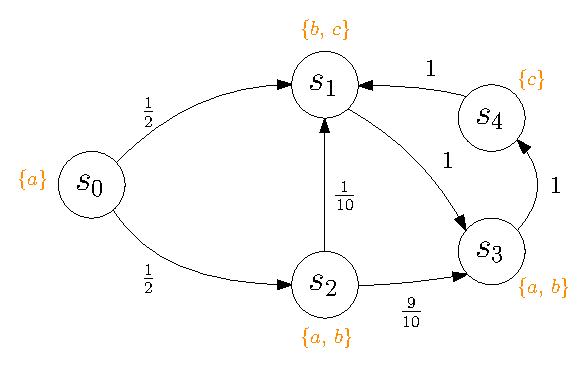
\includegraphics[width=\linewidth]{resources/CUTexample2}
    \captionsetup{justification=centering}
    \captionof{figure}{MC $\mathcal{M}$ with state space $S = \{s_0, s_1, s_2, s_3, s_4\}$ and atomic propositions of the set $AP = \{a, b, c\}$}
    \label{CUTexample2}
  \end{minipage}
    $ \quad $
  \begin{minipage}{0.6\linewidth}
    \centering
    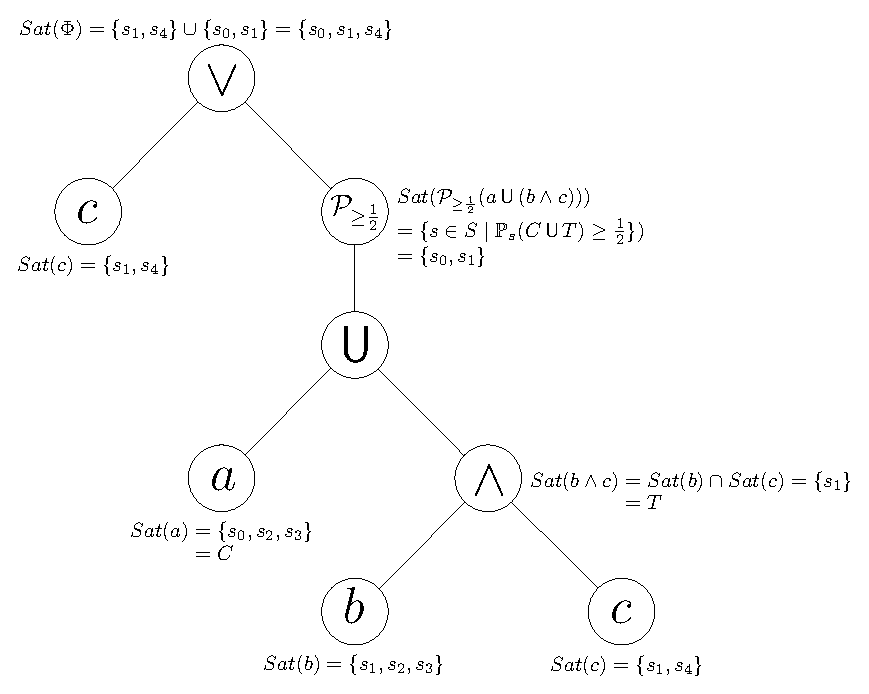
\includegraphics[width=\linewidth]{resources/parse-tree}
    \captionsetup{justification=centering}
    \captionof{figure}{Parse tree of $\mathcal{M}$ for $\Phi$}
    \label{parse-tree-example}
  \end{minipage}
  \end{figure}
  \noindent We are interested to know if $s_0 \models \Phi$. To do that, we build the parse tree of $\Phi$ (cf. Figure \ref{parse-tree-example}).
  We can compute $Sat(\Phi)$ through a bottom up traversal of this tree: we begin at the leaves of the tree, i.e., by computing $Sat(a)$, $Sat(b)$, and $Sat(c)$. Then, we compute $Sat(b \wedge c)$, that equals $Sat(b)\cap Sat(c)$, according to the characterisation of the satisfaction set.
  After that, we compute
  $Sat(\mathcal{P}_{\geq \frac{1}{2}}(a \U (b \wedge c)))$ by computing $\{ s \in S \; | \; \mathbb{P}_s(Sat(a) \U Sat(b \wedge c)) \geq \frac{1}{2}\} = \{ s \in S \; | \; \mathbb{P}_s(\{s_0, s_2, s_3\} \U \{s_1\}) \geq \frac{1}{2}\}$.
  We actually have already computed these probabilities (cf. Example \ref{constrained-reach-example}).
  So, this set equals $\{ s_0, s_1 \}$.
  Finally, from the computation of $Sat(c)$ and $Sat(\mathcal{P}_{\geq \frac{1}{2}}(a \U (b \wedge c)))$, we can compute $Sat(\Phi) = \{s_1, s_4\} \cup \{s_0, s_1\} = \{s_0, s_1, s_4\}$.
  As $s_0 \in Sat(\Phi)$, then $s_0 \models \Phi$.
\end{example}

\section{PCTL for Markov decision processes}
The PCTL syntax for MDPs is almost the same as for MCs with the exception of the probabilistic operator $\mathcal{P}_J(.)$ due to the nondeterminism of MDPs:
we can not verify probabilistic properties without referring to the notion of strategy.
Then, we replace this operator with $\mathcal{P}^{\max}_J(.)$, referring to the probability measure defined on paths of the MC induced by the strategy offering the maximum probability of satisfying a given property.
Thus, the formula $\mathcal{P}^{\max}_J(\phi)$ asserts \[\mathbb{P}^{\max}_s(\{\pi \in Paths(s) \; | \; \pi \models \phi \}) \in J .\]
\textit{Note: $\mathbb{P}_s^{\max}(E)$ refers to the probability measure defined on paths starting from the state $s$ in the MC induced by the strategy maximising the probability of the event $E$ in this MC, i.e., $\max_{\sigma} \mathbb{P}_s^\sigma(E)$.}

\subsection*{Syntax and semantic}

\begin{definition}[\textbf{Syntax of PCTL for MDPs}]
Let $\mathcal{M}$ be an MDP with space of atomic propositions $AP$,
\begin{itemize}
  \item PCTL \textit{state formulae} over $AP$ are formed according to the following grammar:
  \[
    \Phi ::= true \;\; | \;\; a \;\; | \;\; \Phi_1 \wedge \Phi_2 \;\; | \;\; \neg \Phi \;\; | \;\; \mathcal{P}^{\max}_J(\phi)
  \]
  where $a \in AP$ is an atomic proposition, $J \subseteq [0, 1] \cap \mathbb{Q}$ is an interval of probability bounds, and $\phi$ is a path formula.
  \item PCTL \textit{path formulae} over $AP$ are formed according
  to the same grammar as for path formulae in Markov chains context.
\end{itemize}
\end{definition}
\begin{definition}[\textbf{Semantic of PCTL for MDPs}]
  Let $\mathcal{M} = (S, A, \Delta, w, AP, L)$ be an MDP, $s \in S$, $\Phi, \Psi$ be PCTL state formulae over $AP$, and $\phi$ be a PCTL path formula over $AP$,
  \begin{flalign*}
  \intertext{$s \models \Phi$ iff the state formula $\Phi$ holds in the state $s$, i.e.,}
    &\bigcdot\; s \models true, &&&\\
    &\bigcdot\; s \models a &\text{ iff }& a \text{ is a label of $s$, i.e., } a \in L(s),&\\
    &\bigcdot\; s \models \Phi \wedge \Psi &\text{ iff }& s \models \Phi \text{ and } s \models \Psi,&\\
    &\bigcdot\; s \models \neg \Phi &\text{ iff }& s \not\models \Phi, &\\
    &\bigcdot\; s \models \mathcal{P}^{\max}_J(\phi) &\text{ iff }& \mathbb{P}^{\max}_s(\{ \pi \in Paths(s) \; | \; \pi \models \phi \}) \in J.&
  \end{flalign*}
  $\pi \models \phi$ iff the path $\pi$ satisfies $\phi$ in the induced MC.
\end{definition}

\subsection*{Model checking}

PCTL model checking for MDPs is also done almost the same way as for MCs. Indeed, just the characterisation of the satisfiability set $Sat$ is slightly different, due to the semantic of the probabilistic operator $\mathcal{P}^{\max}_J(.)$.
\begin{property}[Characterisation of $Sat$ for MDPs]
Let $\mathcal{M} = (S, A, \Delta, w, AP, L)$ be an MDP, $\Phi, \Psi$ be PCTL state formulae over $AP$, and $\phi$ be a  PCTL path formula over $AP$. The satisfaction set $Sat$ is characterised as follows:
\begin{flalign*}
  Sat(true) &= S,\\
  Sat(a) &= \{s \in S \; | \; a \in L(s)\} \text{ for } a \in AP,\\
  Sat(\Phi) \, \wedge \, Sat(\Psi) &= Sat(\Phi) \cap Sat(\Psi),\\
  Sat(\neg \Phi) &= S \setminus Sat(\Phi), \text{ and} \\
  Sat(\mathcal{P}^{\max}_J(\phi)) &= \{ s \in S \; | \; \mathbb{P}^{\max}_s (Paths(s, \phi)) \in J \} \text{ for } J \subseteq [0, 1] \cap \mathbb{Q},
\end{flalign*}
where $Paths(s, \phi) = \{ \pi \in Paths(s) \; | \; \pi \models \phi \}$.
$\mathcal{P}^{\max}_J(\phi)$ is computed according to the formula $\phi$ as follows:
let $s \in S$ be a state of $\mathcal{M}$,
\begin{flalign*}
  \mathbb{P}^{\max}_s(Paths(s,\, \bigcirc \Phi)) &= \max_{\alpha \in A(s)} \sum_{s' \in Sat(\Phi)} \Delta(s, \alpha, s'), \\
  \mathbb{P}^{\max}_s(Paths(s,\, \Phi \U \Psi)) &= \mathbb{P}^{\max}_s(Sat(\Phi) \U Sat(\Psi)), \text{ and} \tag{cf. Theorem \ref{cut-strategy}}\\
  \mathbb{P}^{\max}_s(Paths(s, \, \Phi \U^{\leq n} \Psi)) &=
    \mathbb{P}^{\max}_s(Sat(\Phi) \U^{\leq n} Sat(\Psi)).
\end{flalign*}
\end{property}

\section{Probabilistic computation tree logic with rewards extension} \label{PRCTL-MC}
To handle properties involving weights of systems, there is a variant of PCTL incorporating the truncated sum function.
This logic is named \textit{probabilistic-reward computation tree logic} (PRCTL, for short).
This logic introduces the expectation operator $\mathcal{E}_C(.)$, and additionally includes the \textit{cost-bounded until} operator $\U_{\leq \ell}$.\\

As for PCTL, we define PRCTL in Markov chains and then describe the slight changes of the syntax and semantic induced by the nondeterminism of Markov decision processes in the following section.

\subsection*{Syntax and semantic}

\begin{definition}[\textbf{Syntax of PRCTL}]
Let $AP$ be a set of atomic propositions,
\begin{itemize}
  \item PRCTL \textit{state formulae} are formed according to the following grammar:
  \[
    \Phi ::= true \;\; | \;\; a \;\; | \;\; \Phi_1 \wedge \Phi_2 \;\; | \;\; \neg \Phi \;\; | \;\; \mathcal{P}_J(\phi) \;\; | \;\; \mathcal{E}_C(\Phi)
  \]
  where $a \in AP$ is an atomic proposition, $J \subseteq [0, 1] \cap \mathbb{Q}$ is an interval of rational bounds, $C \subseteq \mathbb{N} \cup \{+\infty\}$ is an interval of cost bounds, and $\phi$ is a path formula.
  \item PRCTL \textit{path formulae} are formed according to the following grammar:
  \[
  \phi ::= \bigcirc \Phi \;\; | \;\; \Phi_1 \U \Phi_2 \;\; | \;\; \Phi_1 \U^{\leq n} \Phi_2
  \;\; | \;\; \Phi_1 \U_{\leq \ell}\, \Phi_2
  \]
  where $\Phi$, $\Phi_1$ and $\Phi_2$ are state formulae, and $n, \ell \in \mathbb{N}$.
\end{itemize}
\end{definition}
\begin{definition}[\textbf{Semantic of PRCTL}]
  Let $\mathcal{M} = (S, \Delta, w, AP, L)$ be an MC, $s \in S$, $\pi \in Paths(s)$, and $\Phi, \Psi$ be PRCTL state formulae, the semantic of PRCTL is exactly the same as the semantic of PCTL, with the additional expectation operator $\mathcal{E}_C(.)$ and the additional cost bounded operator $\U_{\leq \ell}$, for which the semantic is defined as follows:
  \begin{align*}
  s &\models \mathcal{E}_C(\Phi) &\text{ iff }\quad& \mathbb{E}_s(\TS^{Sat(\Phi)}) \in C,\\
  \pi &\models \Phi \U_{\leq \ell}\, \Psi &\text{ iff }\quad&
  \exists j \in \mathbb{N}, \, s_j \models \Psi, \; \forall i \in \mathbb{N}, \, i<j, \, s_i \models \Phi,
  \text{ and } \TS^{Sat(\Psi)}(\pi) \leq \ell.
  \end{align*}
\end{definition}
%As for the classical constrained and
%step-bounded constrained reachability events, there
%is a cost-bounded constrained reachability event.
 %formed by a countable union of cylinder sets, ensuring the measurability of the event related to the path formula $\Phi \U_{\leq \ell} \Psi$ for state formulae $\Psi$ and $\Phi$ and a cost threshold $\ell$.
%This event is related to the path formula $\Phi \U_{\leq \ell} \Psi$ for state formulae $\Psi$ and $\Phi$ and a cost threshold $\ell$.
%We must thus be sure that this event is measurable in order to ensuring the measurability
%of the event related to the path formula $\Phi \U_{\leq \ell} \Psi$ for state formulae $\Psi$ and $\Phi$ and a cost threshold $\ell$.

In order to ensure the measurability of all events formed by any path formula
$\Phi \U_{\leq \ell}\, \Psi$ for state formulae $\Psi$ and $\Phi$, and a given cost threshold $\ell$,
we define the cost-bounded constrained reachability event as follows.
\begin{definition}[\textbf{Cost-bounded constrained reachability event}]
  Let $\mathcal{M}$ be an MC with state space $S$, $s \in S$, $C, T \subseteq S$, and $\ell \in \mathbb{N}$, the constrained cost-bounded reachability is defined as follows:
    \[
      C \U_{\leq \ell}\, T = \{
        s_0s_1s_2 \dots \in Paths(s) \; | \; \exists n \in \mathbb{N}, \, s_n \in T \, \wedge \, \forall i < n,\, s_i \in C \, \wedge \, \TS^T \leq \ell
      \}.
    \]
\end{definition}

\begin{lemma}[Measurability of cost-bounded constrained reachability events]
  Let $\mathcal{M}$ be an MC with state space $S$,
  $s \in S$, $C, T \subseteq S$, $\ell \in \mathbb{N}$, the event $C \U_{\leq \ell}\, T$ is measurable.
\end{lemma}
\begin{proof2}
  The event $C \U_{\leq \ell} \, T$ is measurable since it can be defined as a countable union of cylinder sets:
    \[C \U_{\leq \ell}\, T = \bigcup_{s_0 \dots s_n \in Paths^{C, \, T}_{\leq \ell}(s)} Cyl(s_0 \dots s_n),
  \]
  where
    $Paths^{C, \,  T}_{\leq \ell}(s)= \{ s_0 \dots s_n \in Paths_{fin}(s) \; | \; \forall i<n,  \, s_i \in C \setminus T \,   \; \wedge \; s_n \in T \; \wedge \; \TS^T(s_0\dots s_n) \leq \ell \}
    $.\\[0.3em]
  $\mathbb{P}_s(C \U_{\leq \ell} \, T)$ denotes the probability of the union of cylinder sets spanned with finite paths of the set $Paths^{C, \, T}_{\leq \ell}(s)$ starting from the state $s \in S$.

\end{proof2}

\subsection*{Model checking}

The PRCTL model checking is also an extension of the PCTL model checking. We just need to describe the changes in the
characterisation of $Sat$ including the new notions introduced in PRCTL.
\begin{property}[PRCTL characterisation of $Sat$]
  Let $\mathcal{M}$ be an MC with state space $S$ and atomic proposition space $AP$, $\Phi$, $\Psi$ be PRCTL state formulae over $AP$ and $\phi$ be a PRCTL path formula over $AP$. The satisfaction set $Sat$ is characterised the same way as in PCTL, with the following additional statements:
  \begin{align*}
    Sat(\mathcal{E}_C(\Phi)) &= \{ s \in S \; | \; \mathbb{E}_s(\TS^{Sat(\Phi)}) \in C \} \text{ for } C \subseteq \mathbb{N} \cup \{+\infty\}, \text{ and} \\
    Sat(\mathcal{P}_J(\phi)) &= \{ s \in S \; | \; \mathbb{P}_s (Paths(s, \phi)) \in J \} \text{ for } J \subseteq [0, 1] \cap \mathbb{Q},
  \end{align*}
    where $Paths(s, \phi) = \{ \pi \in Paths(s) \; | \; \pi \models \phi \}$.
    $\mathcal{P}_J(\phi)$ is computed according to the formula $\phi$ as in PCTL with the following additional statement:
  \[
    \mathbb{P}_s(Paths(s, \Phi \U_{\leq \ell}\, \Psi)) = \mathbb{P}_s(Sat(\Phi) \U_{\leq \ell} \, Sat(\Psi)) \text{ for } s \in S \text{ and } \ell \in \mathbb{N}.
  \]
\end{property}

We already have presented a way to compute $\mathbb{P}_s(\Diamond_{\leq \ell}\, T) = \mathbb{P}_s(S \U_{\leq \ell}\, T)$ for a given state $s \in S$, a set of target states $T \subseteq S$, and a cost threshold $\ell \in \mathbb{N}$ (cf. Theorem \ref{cost-bounded-thm}).
We slightly adapt this method to handle the computation of $\mathbb{P}_s(C \U_{\leq \ell}\, T)$ for $s \in S$, $C, T \subseteq S$, and $\ell \in \mathbb{N}$.
We make all states of $T$ and $S \setminus (C \U T)$ absorbing (cf.  proof of Corollary \ref{qualitative-const-reach}), yiedling a new MC $\mathcal{M}'$.
Then, we build the unfolding of $\mathcal{M}'$ up to $\ell$ (cf. Appendix \ref{app-cbrMC}), i.e., $\mathcal{M}'_{\ell}$.
We finally resolve a classical cost-bounded reachability (i.e., $C \U T$) in $\mathcal{M}'_{\ell}$.

\begin{example}[\textit{PRCTL model checking: expectation operator}]
  Let $\mathcal{M}$ be the MC with state space $S$ and atomic proposition space $AP$ of Figure \ref{CUTexample3}, and the state formula $\Phi = \mathcal{E}_{\leq{5}}(c \vee \mathcal{P}_{\geq \frac{1}{2}}(a \U (b \wedge c)))$.
  \begin{figure}[h]
    \centering
    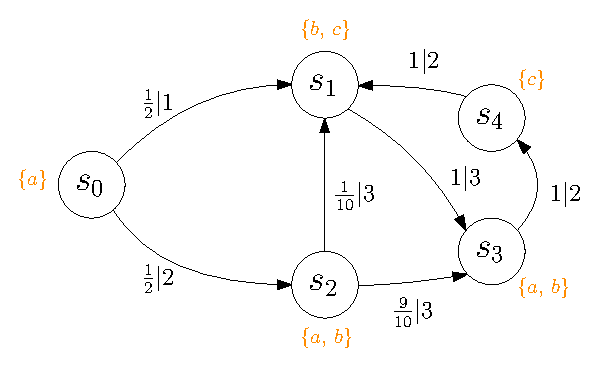
\includegraphics[width=0.5\linewidth]{resources/CUTexample3}
    \captionsetup{justification=centering}
    \caption{MC $\mathcal{M}$ with state space $S = \{s_0, s_1, s_2, s_3, s_4\}$ and atomic propositions of the set $AP = \{a, b, c\}$}
    \label{CUTexample3}
  \end{figure}
  We are interested to know if $s_2 \models \Phi$.
  Let $\Psi = c \vee \mathcal{P}_{\geq \frac{1}{2}}(a \U (b \wedge c)))$.
  So, we compute $Sat(\mathcal{E}_{\leq 5}(\Psi)) = \{s \in S \; | \; \mathbb{E}_s(\TS^{Sat(\Psi)}) \leq 5\}$. The set $Sat(\Psi)$
  has already been computed in Example \ref{exCUT}.
  Then, the set $Sat(\mathcal{E}_{\leq 5}(\Psi)) = \{s \in S \;|\; \mathbb{E}_s(\TS^{\{s_0, s_1, s_4\}})\leq 5\}$.
  We can compute
  $\mathbb{E}_s(\TS^{\{s_0, s_1, s_4\}})$ for all $s \in S$, according to the equation system defined in Appendix \ref{app-expMC}.
  Let $S_{=?} = \{ s \in S \; | \; \mathbb{P}_s(\Diamond \{s_0, s_1, s_4\}) = 1 \} \setminus \{s_0, s_1, s_4\} =
  \{s_2, s_3\}$ and $(x_s)_{s \in S} \in [0, 1]^{|S|}$ such that $x_s = \mathbb{E}_s(\TS^{\{s_0, s_1, s_4\}})$ for all $s \in S$, we firstly have $x_{s_0} = x_{s_1} = x_{s_4} = 0$.
  We additionally have
  \begin{align*}
    \begin{pmatrix}
      x_{s_2}\\[0.3em]
      x_{s_3}
  	\end{pmatrix} &=
    \begin{pmatrix}
      0 & \frac{9}{10} \\[0.3em]
      0  & 0
    \end{pmatrix}
    \begin{pmatrix}
      x_{s_2}\\[0.3em]
      x_{s_3}
  	\end{pmatrix}
    +
    \begin{pmatrix}
      \frac{3}{10}\\[0.3em]
      2
    \end{pmatrix},
  \end{align*}
  and we thus have $x_{s_3} = \mathbb{E}_{s_3}(\TS^{\{s_0, s_1, s_4\}}) = 2 \leq 5$ and $
    x_{s_2} = \mathbb{E}_{s_2}(\TS^{\{s_0, s_1, s_4\}}) = \frac{9}{10} (x_{s_3} + 3) + \frac{3}{10}
    = \frac{9}{10} \cdot 5 + \frac{3}{10}
    = \frac{48}{10}\leq 5$. Then, $Sat(\mathcal{E}_{\leq 5}(\Psi)) = S$ what implies $s_2 \models \Phi$.
\end{example}

\section{PRCTL for Markov decision processes}\label{PRCTL-MDP}
Again, PRCTL for Markov decision processes is slightly different than PRCTL for Markov Chains.
We need to adapt the syntax and the semantic of PRCTL for Markov chains in order to support nondeterminism induced by Markov Decision processes.
Indeed, in addition to the probabilistic operator $\mathcal{P}_J(.)$ that changes to $\mathcal{P}_J^{\max}(.)$ for the same reason as in PCTL,
the expectation operator $\mathcal{E}_C(.)$ becomes ambiguous for Markov decision processes due to nondeterminism.
In Markov chains, this operator directly refers to the expected cost to reach a set of target states.
We cannot address the expect cost-to-target in Markov decision process without referring to the notion of strategies.
Then, we replace this operator with $\mathcal{E}^{\min}_C(.)$, referring to the expected cost-to-target in the Markov chain induced by the strategy minimising this cost in the MDP.

\subsection*{Syntax and semantic}

\begin{definition}[\textbf{Syntax of PRCTL for MDPs}]
Let $\mathcal{M}$ be an MDP with space of atomic propositions $AP$,
\begin{itemize}
  \item PRCTL \textit{state formulae} over $AP$ are formed according to the following grammar:
  \[
    \Phi ::= true \;\; | \;\; a \;\; | \;\; \Phi_1 \wedge \Phi_2 \;\; | \;\; \neg \Phi \;\; | \;\; \mathcal{P}^{\max}_J(\phi) \;\; | \;\; \mathcal{E}^{\min}_C(\Phi)
  \]
  where $a \in AP$ is an atomic proposition, $J \subseteq [0, 1] \cap \mathbb{Q}$ is an interval of probability bounds, $C \subseteq \mathbb{N} \cup \{+\infty\}$ gives cost bounds, and $\phi$ is a path formula.
  \item PRCTL \textit{path formulae} over $AP$ are formed according to the same grammar as for PRCTL path formulae in Markov chains context.
\end{itemize}
\end{definition}
\begin{definition}[\textbf{Semantic of PRCTL for MDPs}]
  Let $\mathcal{M}$ be an MDP with state space $S$, $s \in S$ and atomic proposition space $AP$, and $\Phi$ be a PRCTL state formula over $AP$,
  the semantic of PRCTL state formulae for MDPs is exactly the same as the PCTL state formulae semantic for MDPs, with the additional expectation operator $\mathcal{E}^{\min}_C(.)$ for which the semantic is defined as follows:
  \[
  s \models \mathcal{E}^{\min}_C(\Phi) \quad \text{ iff }\quad \mathbb{E}^{\min}_s(\TS^{Sat(\Phi)}) \in C.
  \]
  The PRCTL semantic of paths formulae for MDPs is the same as the PRCTL semantic of paths formulae for MCs.
\end{definition}

\subsection*{Model checking}

As the PRCTL model checking is done
through the recursive computation of the satisfaction set, we just need to slightly adapt the characterisation of the PCTL satisfiability set for MDPs.
\begin{property}[PRCTL characterisation of $Sat$ for MDPs]
  Let \sloppy$\mathcal{M}$ be an MDP with state space $S$ and atomic proposition space $AP$, $\Phi$, $\Psi$ be PRCTL state formulae over $AP$, and $\phi$ be a PRCTL path formula over $AP$. The satisfaction set $Sat$ is characterised the same way as in PCTL, with the following additional statements:
  \begin{align*}
    Sat(\mathcal{E}^{\min}_C(\Phi)) &= \{ s \in S \; | \; \mathbb{E}^{\min}_s(\TS^{Sat(\Phi)}) \in C \} \text{ for } C \subseteq \mathbb{N} \cup \{+\infty\}, \text{ and} \\
    Sat(\mathcal{P}^{\max}_J(\phi)) &= \{ s \in S \; | \; \mathbb{P}^{\max}_s (Paths(s, \phi)) \in J \} \text{ for } J \subseteq [0, 1] \cap \mathbb{Q},
  \end{align*}
    where $Paths(s, \phi) = \{ \pi \in Paths(s) \; | \; \pi \models \phi \}$.
    $\mathcal{P}^{\max}_J(\phi)$ is computed according to the formula $\phi$ as in PCTL, with the following additional statement:
  \[
    \mathbb{P}^{\max}_s(Paths(s, \Phi \U_{\leq \ell}\, \Psi)) = \mathbb{P}^{\max}_s(Sat(\Phi) \U_{\leq \ell} \, Sat(\Psi)) \text{ for } s \in S \text{ and } \ell \in \mathbb{N}.
  \]
\end{property}

%In order to compute the maximum probability of paths formed by a cost-bounded constrained path formula (i.e., a path formula of the form $\Phi \U_{\leq \ell} \, \Psi$),
We compute $\mathbb{P}_s^{\max}(C \U_{\leq \ell} \, T)$ for a given state $s$ of the system, $C, T \subseteq S$, and $\ell \in \mathbb{N}$, by reduction to the cost-bounded reachability to $T$ the same way as we compute the classical constrained reachability by reduction to the reachability to $T$ (cf. proof of Theorem \ref{cut-strategy}).
We make all states $s^* \in S \setminus (C \cup T)$ absorbing, i.e., we replace all enabled actions in $A(s^*)$
by a unique action $\alpha_{s^*}$ such that $\Delta(s^*, \alpha_{s^*}, s^*) = 1$.
Then, we compute $\mathbb{P}^{\max}_s(\Diamond_{\leq \ell}\, T)$ in this modified MDP and we build the linked strategy, corresponding to the optimal strategy built for the \SSPP{} problem for the state $s$, the subset of target states $T$, the cost threshold $\ell$, and an arbitrary probability threshold (cf. Theorem \ref{sspp-thm}).

\begin{remark}[\textit{Value iteration for the minimal expected cost-to-target}]
  The equation system in Appendix \ref{bellman2} suggests an approximation technique, called value iteration to compute the minimal expected cost-to-target in an MDP.
  This value iteration technique can be defined in a similar way as for maximising the probability to reach this target (cf. Theorem \ref{bellman1}).
\end{remark}

\begin{remark}[\textit{PRCTL model checking and \SSPE{} problem}]
  Let $\mathcal{M}$ be an MDP with state space $S$ and atomic proposition space $AP$, $s \in S$, $\ell \in \mathbb{N}$, and $\Phi$ be a PRCTL state formula over $AP$,
  verify $s \models \mathcal{E}^{\min}_{\leq \ell}(\Phi)$ is equivalent to solve the \SSPE{} problem for the state $s$, the cost threshold $\ell$ and the subset of target states $Sat(\Phi)$.
\end{remark}
\begin{remark}[\textit{PRCTL model checking and \SSPP{} problem}]
  Let \sloppy$\mathcal{M}$ be an MDP with state space $S$ and atomic proposition space $AP$, $s \in S$, $\ell \in \mathbb{N}$, $\alpha \in [0, 1] \cap \mathbb{Q}$, and $\Phi$ be a PRCTL state formula over $AP$,
  verify $s \models \mathcal{P}^{\max}_{\geq \alpha}(\Diamond_{\leq \ell}\, \Phi)$ is equivalent to solve the \SSPP{} problem for the state $s$, the cost threshold $l$, the probability threshold $\alpha$ and the set of target states $Sat(\Phi)$.
\end{remark}

\begin{example}[\textit{PRCTL model checking: cost-bounded until operator}] \label{cost-bounded-example}
Let $\mathcal{M} = (S, A, \Delta, w, AP, L)$ be the MDP of Figure \ref{cost-bounded-until1}, we are interested in verifying $s_0 \models \mathcal{P}^{\max}_{\geq \frac{1}{5}}((a \vee b) \U_{\leq 8} \, c)$.
\begin{figure}[h]
  \centering
  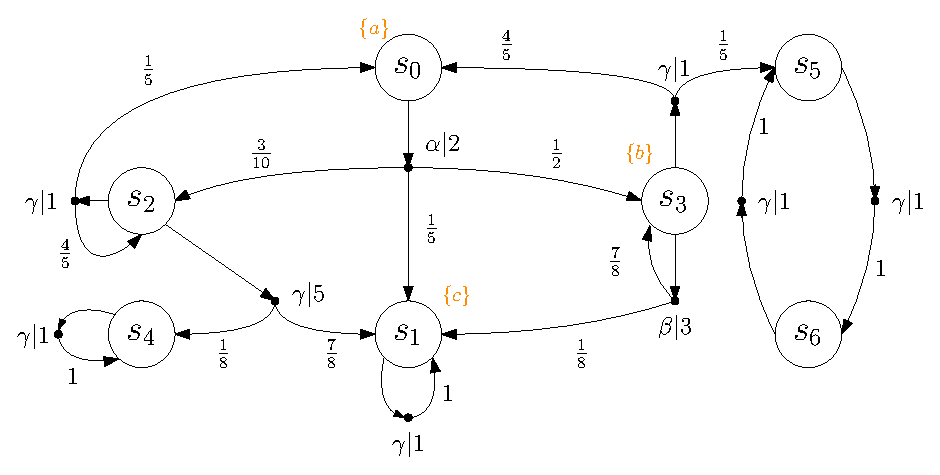
\includegraphics[width=0.7\linewidth]{resources/MDPExample}
  \captionsetup{justification=centering}
  \caption{MDP $\mathcal{M}$, with state space $S=\{s_0, s_1, s_2, s_3, s_4, s_5, s_5\}$ and with space of atomic propositions $AP = \{a, b, c\}$}
  \label{cost-bounded-until1}
\end{figure}
First, we begin by computing the sets $Sat(a \vee b)$ and $Sat(c)$. Let $C = Sat(a \vee b)$ and $T = Sat(c)$. We have $C = \{s_0, s_3\}$ and $T = \{ s_1 \}$.
Then, we make all states of the set $S \setminus (C \cup T)$ absorbing, i.e., all states of $\{s_2, s_4, s_5, s_6\}$ (cf. Figure \ref{cost-bounded-until2}), to set up the reduction of this problem to the cost-bounded reachability to $T$.
\begin{figure}[h]
  \centering
  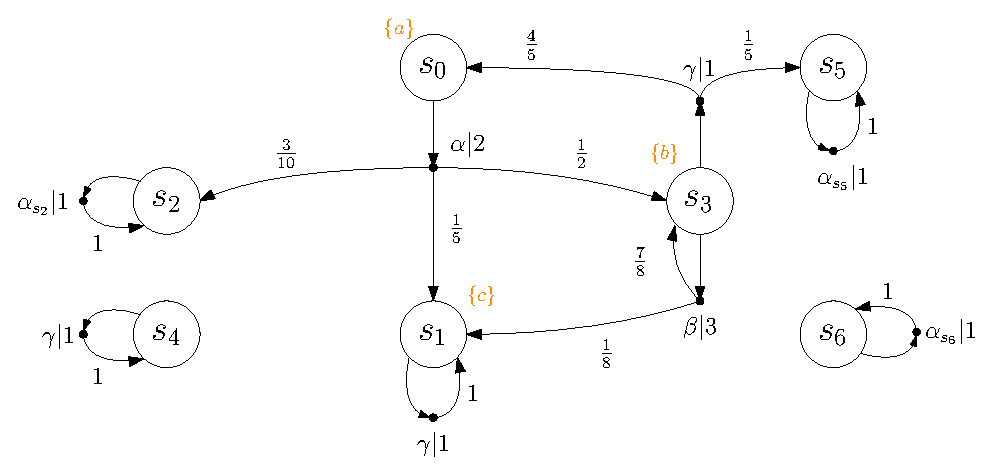
\includegraphics[width=0.7\linewidth]{resources/MDPExample2}
  \captionsetup{justification=centering}
  \caption{MDP $\mathcal{M}$ modified to verify the property $\mathcal{P}^{\max}_{\geq \frac{1}{5}}((a \vee b) \U_{\leq 8} \, c)$ by reduction to the cost-bounded reachability to $T$}
  \label{cost-bounded-until2}
\end{figure}
Now, it remains to compute $\mathbb{P}_{s_0}^{\max}(\Diamond_{\leq 8} \, T)$ in the modified MDP.
To do that, we unfold it from the state $s_0$ up to the cost threshold $\ell=8$ (cf. Figure \ref{cost-bounded-until3}).
\begin{figure}[h]
  \centering
  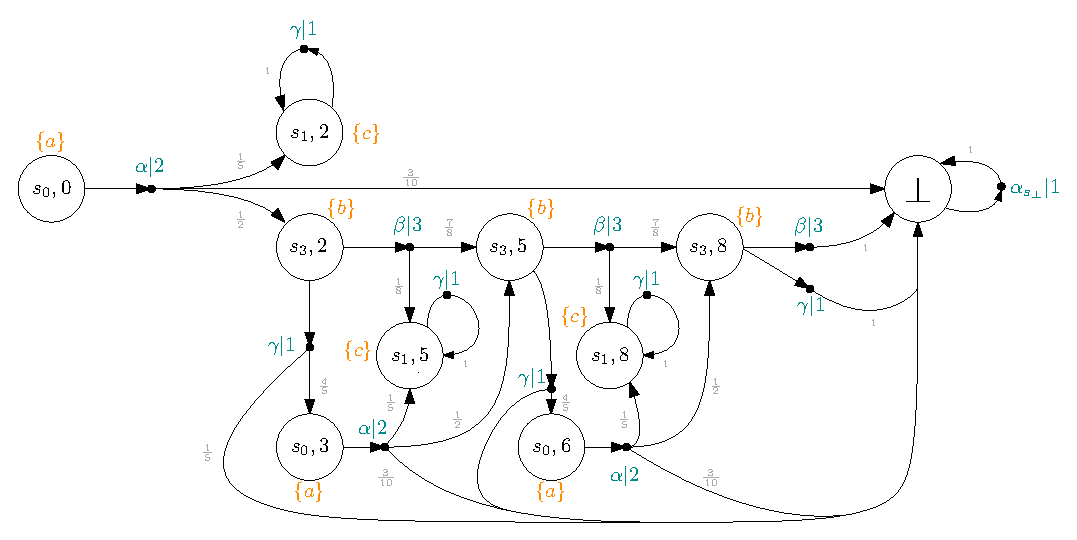
\includegraphics[width=0.9\linewidth]{resources/MDPExample-unfolded}
  \captionsetup{justification=centering}
  \caption{Unfolding of the modified MDP from the state $s_0$ up to the cost threshold $\ell=8$}
  \label{cost-bounded-until3}
\end{figure}
\end{example}
Let $S_\ell$ be the state space of the unfolding of $\mathcal{M}$ and $T_\ell = \{(s_1, 2), (s_1, 5), (s_1, 8)\} $
be the new set of target states.
We compute $\mathbb{P}^{\max}_{(s_0, 0)}(\Diamond \, T_{\ell})$ in this unfolding of $\mathcal{M}$ according to the linear program defined in Appendix \ref{app-sr}: let $(x_{(s, v)})_{(s, v) \in S_{\ell}} \in [0, 1]^{|S_{\ell}|}$ such that $x_{(s, v)} = \mathbb{P}^{\max}_{(s, v)}(\Diamond T_\ell)$ for all $(s, v) \in S_\ell$.
We have $x_{s_\bot} = x_{(s_3, 8)} = 0$
because $s_{\bot}$ and $(s_3, 8)$ are not connected to $T_\ell$ and $x_t = 1$ for all $t \in T_\ell$. Then, the vector $(x_s)_{s \in S_\ell}$ is the unique solution of the following linear program:
\begin{align*}
\intertext{\centering $\min \, x_{(s_0,0)} + x_{(s_0,3)} + x_{(s_0,6)} + x_{(s_3,2)} + x_{(s_3,5)}$}\\
\intertext{subject to}
  x_{(s_0,0)} - \tfrac{1}{2} x_{(s_3,2)} &\geq \tfrac{1}{5} &
  x_{(s_3,2)} - \tfrac{7}{8} x_{(s_3,5)} &\geq \tfrac{1}{8}\\
  - \tfrac{4}{5} x_{(s_0,3)} + x_{(s3,2)} &\geq 0 &
  x_{(s_3,5)} &\geq \tfrac{1}{8}\\
  - \tfrac{4}{5} x_{(s_0,6)} + x_{(s_3,5)} &\geq 0 &
  x_{(s_0,6)} &\geq \tfrac{1}{5}\\
  x_{(s_0,3)} - \tfrac{1}{2} x_{(s_3,5)} &\geq \tfrac{1}{5} && & \\[1em]
  0 \leq x_{(s_0,0)} &\leq 1 &
  0 \leq x_{(s_0,3)} &\leq 1 \\
  0 \leq x_{(s_0,6)} &\leq 1 &
  0 \leq x_{(s_3,2)} &\leq 1 \\
  0 \leq x_{(s_3,5)} &\leq 1 & &
\end{align*}
We can solve this linear program via the simplex method. This yields ${x_{(s_0, 0)}=0.3325}$. Since $x_{(s_0, 0)} = \mathbb{P}_{(s_0, 0)}^{\max}(\Diamond T_\ell) = \mathbb{P}^{\max}_{s_0} (\Diamond_{\leq 8}\, T)$ in the modified MDP, we have that $x_{(s_0, 0)} = \mathbb{P}^{\max}_{s_0}(C \U_{\leq 8} \, T)$ in
$\mathcal{M}$, and $x_{(s_0, 0)} \geq \frac{1}{5}$. Then, $s_0 \models \mathcal{P}_{\geq \frac{1}{5}}^{\max}((a \vee b) \U_{\leq 8}\, c)$.
